\documentclass[11pt,a4paper]{article}
\usepackage[a4paper,bindingoffset=0.2in,left=1in,right=1in,top=1in,bottom=1in,footskip=.25in]{geometry}

\usepackage{amsmath}
\usepackage{amsfonts}
\usepackage{makeidx}
\usepackage{amssymb}
\usepackage{hyperref}
\usepackage{graphicx}
\usepackage{caption}
\usepackage{float}
\usepackage{indentfirst}
\usepackage[utf8]{inputenc}
\usepackage[normalem]{ulem}
\usepackage[spanish,es-tabla]{babel}
\useunder{\uline}{\ul}{}
\usepackage{afterpage}

% \captionsetup[figure]{font=small,skip=-5pt}

\title{Sistemas de Inteligencia Artificial\\Redes Neuronales\\Trabajo Práctico Especial Número 2}
\date{Junio 2015}
\author{Federico Tedin - 53048\\Javier Fraire - 53023\\Ignacio Rivera - 53029}

\makeindex

\begin{document}
\maketitle
\thispagestyle{empty}

\vspace{5mm}
\renewcommand{\abstractname}{Resumen:}
\begin{abstract}

\centering
Implementar una red neuronal multicapa con aprendizaje supervisado que estime la siguiente función:
$$ y = sin(x) \times x^3 + \frac{x}{2}, \ \text{con} \ x \ \epsilon \ [10, 45] $$
\end{abstract}

\clearpage

\renewcommand{\contentsname}{Índice}
\tableofcontents
\thispagestyle{empty}
\clearpage
\setcounter{page}{1}

\section{Introducción}
\subsection{Objetivo}

El objetivo del trabajo práctico realizado fue implementar una red neuronal multicapa con aprendizaje supervisado que estime la funcion:

$$ f(x) = sin(x) \times x^3 + \frac{x}{2}, \ \text{con} \ x \ \epsilon \ [10, 45] $$

El propósito de la red neruonal es, mediante el algoritmo \emph{backpropagation}, modificar los pesos que conectan las neuronas de manera que cuando se corra el \emph{feed forward} el error cuadrático medio sea menor que una cota dada.

\subsection{Aclaraciones}

Para todas las pruebas realizadas se utilizó el mismo \emph{seed} para generar los números aleatorios. De esta forma, las pruebas son más fieles ya que parten del mismo estado inicial. Además, así se evitó tener correr múltiples pruebas para determinados parámetros ya que el resultado es el mismo. 

En todas las pruebas se normalizó la salida para evitar tener que usar unícamente una función lineal en la capa de salida y poder utilizar cualquier función de activación.

Para el cálculo del error cuadrático médio se utilizo la siguiente fórmula:

$$E(W) = \frac{1}{n} \sum_{\mu i}{(S_i^{\mu} - o_i^{\mu})^2}$$

, donde $n$ es la cantidad de patrones.

Se estableció $0.0001$ como error cuadrático medio de corte.

En todas las pruebas el incremento en el intervalo utilizado es de $0.5$. Se tomó esta decisión ya que con este incremento las pruebas se realizaban más rápido, por lo que se podían correr más pruebas. Además se observó que con este intervalo se logra obtener una buena aproximación.

\section{Correcciones}

La implementación en la entrega anterior no funcionaba correctamente. No lograba aproximar bien la función y los gráficos no eran precisos. Revisando la implementación se encontró un error. Al momento de calcular el error cuadrático medio y al momento de graficar la función no se corría un \emph{feed forward} de la red por lo que las salidas calculadas habían utilizado pesos distintos, y no el obtenido al pasar el último patrón. Por lo tanto el algoritmo funcionaba correctamente pero se estaba calculando mal error cuadrático medio y se estaba mostrando mal la función.

Una vez corregido el error anterior, se procedió a probar con la arquitectura recomendada por la cátedra (\emph{1-35-10-1}). Se realizaron diversas pruebas utilizando distintos valores de $\beta$. Estas pruebas no resultaron exitosas. Se puede apreciar en la figura \ref{fig:sinNormalizar} que se obtenía una línea recta. Analizando las capas ocultas se observaba que si el beta era muy ``grande'' ($\beta \geq 0.3$) se producía una saturación de las neuronas. Esto se debe a que los patrones de entrada son números muy grandes, lo que ocasionaba que la suma pesada de los patrones por los pesos diera muy grande. Esto causaba que la función de activación de un valor cercano a |$1$|. Por esta razón se procedió a probar con $\beta$ más pequeños. Se observaron las salidas de las capas ocultas y se pudo apreciar que los valores eran muy similares por lo que la red no podía diferenciarlos.

Debido a que no se lograba aproximar la función correctamente y utilizando los resultados anteriores, se decidió normalizar la entrada, es decir, cambiar la representación de los patrones. Al normalizar, se trabajó con números más pequeños evitando la saturación de las neuronas, ya que la suma pesada de los pesos por los patrones tenía como resultado valores más acotados. El problema que se encontró al normalizar es que los patrones tenían valores muy pequeños y más difíciles de difrenciar, ya que se pasó del intervalo $[10,45]$ al intervalo $[-1,1]$. Al utilizar $\beta = 1$ la red se encontraba con dificultades al diferenciar los patrones, por lo que no se obtuvo una aproximación correcta. Entonces, se decidió probar con valores de $\beta$ más grande. Esto si resultó exitoso ya que con un valor de $\beta$ más grande la red logró diferenciar mejor los patrones. Los resultados de dichas pruebas y su análisis se encuentran en al siguiente sección.

\section{Pruebas y análisis}
\subsection{Primeras pruebas}

Como se mencióno en la sección anterior, primero se probó utilizando $\beta = 1$. Los resultados de dicha prueba se encuentran en la figura \ref{fig:PruebaRecu11}. Esta prueba no resultó exitosa.
 
Luego, se probó la misma arquitectura pero utilizando $\beta = 3$. Como se puede observar en la figura \ref{fig:pruebaRecu1} esta prueba resultó exitosa, es decir, se logró obtener una aproximación aceptable de la función. Como se mencionó anteriormente, esto se debe a que le permite  a la red diferenciar más los patrones. Luego, se probó cambiar la función de activación de la capa de salida por la función tangencial. El resultado se encuentra en la figura \ref{fig:pruebaRecu15} y este fue mejor que en la prueba anterior. Analizando el gráfico, se puede observar como logra aproximar más precisamente los valores más grandes, es decir, el sector derecho del gráfico. Esto se debe a que al ser valores más grandes la red logra diferenciarlos mejor. En el intervalo $[-1, -0.2]$ la función se encuentra entre $-0.1$ y $0.1$ mientras que en el intevalo $[0.2, 1]$ entre $-1$ y $1$ y ambos intervalos tienen la misma cantidad de puntos, por lo que la diferencia entre los patrones del menor intervalo es mucho menor. A su vez, se observa que si bien no logra aproximar correctamente la función en  el intervalo $[- 0.2, -1]$ el error cuadrático medio es bajo. Esto se debe a que los valores de salida en dicho interavalo son muy pequeños por lo que la diferencia entre la salida calculada y la esperada es pequeña. Análogamente, el intervalo $[-0.2, 1]$ tiene una mayor importancia en el error cuadrático medio y al aproximar dicho intervalo de la función se obtiene un error cuadrático medio bajo.

\subsection{Pruebas de distintas arquitecturas}


Una vez que se logró obtener una aproximación aceptable de la función, se procedió a probar distintas arquitecturas para observar como se comportaban. Se probaron las arquitecturas \emph{1-35-10-1}, \emph{1-35-15-1}, \emph{1-35-20-1} y \emph{1-35-1}. En la tabla \ref{table:pruebaArqs} se encuentran los resultados. Se realizaron cuatro pruebas con cada arquitectura (en todas menos la última arquitectura) utilizando los mismos parámetros. Se utilizaron los mismos parámetros para que las pruebas sean lo más fieles posible. Ló único que se varió fue la función de activación. En la tabla \ref{table:pruebaArqs} se observa que la arquitectura \emph{1-35-10-15} fue inferior en todas las pruebas con arquitecturas de dos capas ocultas ya que obtuvo un error cúadratico medio menor que el resto de las arquitecturas (en algunos casos hasta un orden de magnitud menor). En cuanto a las otras dos arquitecturas de dos capas, sus resultados fueron variados. Comparando las pruebas 7 y 11 y las pruebas 8 y 12, se observa que la arquitectura \emph{1-35-15-1} fue superior al obtener un error cuadrático medio más bajo. Pero al comparar las pruebas 5 y 9 y 6 y 10, se observa que la arquitectura \emph{1-35-20-1} fue superior. Dados estos resultados se eligió como arquitectura óptima a la arquitecutra \emph{1-35-15-1} ya que probó ser mejor que la arquitectura \emph{1-35-10-1} y que no se encontró una diferencia notable con la arquitectura \emph{1-35-20-1}. Además, la arquitecura elegida tiene menos neuronas, por lo que requiere un menor poder de procesamiento que la arquitectura \emph{1-35-20-1}. La razón por la que la aquitectura elegida es superior a la arquitectura \emph{1-35-10-1} es que al tener un mayor número de neuronas en la segunda capa oculta, la red puede distinguir mejor los patrones por lo que puede aproximar mejor el sector izquierdo de la función. Esto se puede observar en la figura \ref{fig:pruebaRecu10}. La prueba anterior, también sirvió para determinar que función de activación resultaba mejor. En la tabla \ref{table:pruebaArqs} se puede observar que en todos los casos la función exponencial resultó inferior. Por este motivo, se decidió omitir probar ésta en la capa de salida. Además de elegir la arquitectura, se decidió utilizar la función tangencial en las capas ocultas y la función lineal en las capa de salida, ya que fue la mejor combinación para la arquitectura elegida. También, se puede observar que utilizar una única capa no arrojo buenos resultados. En la prueba 13 de la tabla \ref{table:pruebaArqs} se puede observar que el error cuadrático medio es muy superior al resto de los errores. Se puede observar que le falta una segunda capa oculta para poder diferenciar mejor los patrones. En la figura \ref{fig:unaCapa}, se puede ver que esta no es una buena aproximación.

\subsection{Variaciones de la tasa de aprendizaje}
Una vez elegida la estructura que se utilizó para el resto de las pruebas, se comenzó a variar los diferentes parámetros que alteran el funcionamiento de la red neuronal en pos de encontrar los mejores para el problema definido. Se comenzó variando el valor de la tasa de aprendizaje ($\eta$). Durante las pruebas mencionadas en el inciso anterior se utilizó como valor de este paráametro $\eta = 0.001$, ya que por la naturaleza de nuestros patrones y la salida de estos, se necesita que el $\eta$ sea relativamente bajo para que el aprendizaje, que viene dado por la modificación en los pesos, se haga de a pequeños pasos para asegurar presición. Los resultados de esta prueba se encuentran en la tabla \ref{table:pruebaEta}. Lo primero que es importante a destacar de esta prueba es cómo el error tiene pocas oscilaciones y tiende a ser siempre decreciente. Esto se debe a que como el valor de $\eta$ es pequeño el aprendizaje tiende a ser un poco más lento pero más uniforme. Por el otro lado tomando $\eta = 0.005$, cinco veces más grande que el anterior, podemos ver en la figura \ref{fig:pruebaRecu29} cómo en las primeras épocas error tiende a oscilar más que en la figura \ref{fig:pruebaRecu10}. Un análisis similar se puede hacer cuando se usa $\eta = 0.0005$, el error tiene pocas oscilaciones pero el aprendizaje resulta ser más lento que con $\eta =  0.001$. Esto se puede observar en la tabla \ref{table:pruebaEta} en las pruebas 2 y 3, donde en la primera de estas llega a la mitad del error en la misma cantidad de epocas. No obstante, como se puede observar en la tabla \ref{table:pruebaEta}, en la entrada 1 que corresponde a la figura \ref{fig:pruebaRecu29} el error obtenido con esta tasa de aprendizaje es mucho menor que con $\eta = 0.001$ y termina incluso antes de las $5000$ epocas. Es decir, por primera vez se llega al error caudrático medio mínimo establecido. Dado estos resultados y que las osilaciones en el error se vuelven despreciables a medida que las epocas avanzan y el error disminuye, se eligio seguir las pruebas con $\eta = 0.005$. 

\subsection{Variaciones de \texorpdfstring{$\beta$}{\emph{beta}}}

Después de encontrar un buen valor de $\eta$ se probaron distintos valores de $\beta$ con el fin de encontrar si había alguno mejor. En la tabla \ref{table:pruebaBeta} se encuentran los resultados. En la misma se puede observar que ninguna prueba arrojó mejores resultados que el valor de $\beta$ utilizado anteriormente ($\beta = 0.3$). En el caso de las pruebas 2 y 3 se debe a que a medida que se incrementa el beta, la función de activación tiende a la función escalón por lo que su salida da valores menos distingubles y más cercanos a $|1|$. Por ello, a la red le cuesta más aprender. En el caso de la prueba 1, ésta arrojó peores resultados porque $\beta$ no es lo suficientemente grande como para que la red pueda distinguir bien los patrones. Debido a los resultados obtenidos en estas pruebas, se decidió utilizar $\beta = 3$ para el resto de las pruebas.

\subsection{Momentum}
Una de las mejoras que se implementó fue el uso de \emph{momentum} a la hora de hacer las modificaciones de pesos. Para estas pruebas se utilizo como tasa de aprendizaje $\eta = 0.005$. Se probaron distintos valores de $\alpha$ para el \emph{momentum} para poder descubrir, dados nuestros parámetros, cuál era el mejor valor de $\alpha$ para correr esta mejora. En la tabla \ref{table:pruebaMomentum} se puede observar que la prueba que arrojó los mejores resultados fue la prueba 2 ($\alpha = 0.3$). Cuando la red se encuentra en un \emph{plateau} de la superficie de corte la tasa de aprendizaje efeciva es $\frac{\eta}{1 - \alpha}$. Por este motivo, las pruebas que utilizaron un $\alpha$ mayor resultaron inferiores. Cuanto mayor es $\alpha$, menor es el coeficiente que se encuentra dividiendo por lo que $\eta$ es mayor y el error tiende a oscilar más. Estás diferencias en las oscilaciones del error se pueden observar en las figuras \ref{fig:pruebaRecu40}, \ref{fig:pruebaRecu25}, \ref{fig:pruebaRecu26}, \ref{fig:pruebaRecu27} y \ref{fig:pruebaRecu28}. Se observa en la figura \ref{fig:pruebaRecu28} cómo un con un $\alpha = 0.9$ las oscilaciones son muy grandes y como se van reduciendo en el resto de las figuras.  A su vez,  $\alpha = 0.2$ menor resultó ser menos efectivo que $\alpha = 0.3$. Esto se debe a que hay que encontrar un punto medio en el que las oscilaciones no sean muy grandes pero que no sean demasiado pequeñas. Es decir, deben ser lo suficientemente grandes como para ayudar a la red a salir del \emph{pleateau} pero no tan grandes como para causar que el error oscile demasiado. Además, se observa que no solo utilizar mayores valores de $\alpha$ arrojó peores resultados que utilizando menores valores, sino que también arrojó peores resultados que no utilizar la mejora. Por lo tanto, \emph{momentum} es una gran mejora pero depende de los parámetros empleados. 
   
   
\subsection{\texorpdfstring{$\eta$ adaptativo}{Tasa de aprendizaje adaptativa}}

Una vez realizadas las pruebas de \emph{momentum}, se procedió a realizar pruebas con $\eta$ adaptativo. Como se puede observar en la tabla \ref{fig:pruebaRecu39}, no se consiguió obtener mejores resultados que no utilizando la mejora. Esto no significa que la mejora no funcione o no este correctamente implementada, significa que no se encontraron las parámetros adecuados para lograr un mejor resultado. Las combinaciones de estos paramétros son infinitas por lo que es posible que no se encuentren los óptimos. Sin embargo, se puede observar que a diferencia de utilizar \emph{momentum} o de no utilizar ninguna mejora, el error cuadrático medio es siempre decreciente por lo que, si se corriese una prueba con esta mejora en un tiempo mucho más prolongado, la mejora $\eta$ adaptativo difícilmente se estancaría en un \emph{pleateau} mientras que en los otros casos es más probable. El hecho de que $\eta$ se ajuste a lo largo del tiempo garantiza que el error continurá decreciendo. En la figura \ref{fig:pruebaRecu39} se puede observar el gráfico de la mejor prueba (4). Además, se puede ver que en la mayoría de los casos el valor de $\eta_final$ es muy similar por lo que se puede inferir que sin importar los parámetros que se utilicen, eventualmente la red alcanzará un $\eta$ similar. Otra razón por la que puede no haber funcionado efectivamente es que la red se entrenó utilizando \emph{incremental} y $\eta$ adaptativo se implementó por época por lo que pasan por lo menos $n$ actualizaciones de peso entre cada modificación de $\eta$. Entonces, le puede costar mucho a la red realizar un paso positivo. Esto causa que funcione más lento.

\subsection{Combinación de las mejoras}

Luego, se tomaron los mejores el resultados de la prueba anterior y el mejor resultado de las pruebas de \emph{momentum} y se corrió una combinación de ambos. Como se puede observar en la tabla \ref{table:pruebaComb} todas las pruebas obtuvieron peores resultados que utilizando sólo $\eta$ adaptativo. Esto se debe, a que no se encontró la combinación de parámetros correcta.  Como \emph{momentum} cambia el funcionamiento de la red, puede ser que los parámetros para $\eta$ adaptativo deban ser diferentes. A su vez, arrojó peores resultados que utilizando solo \emph{momentum} o sin utilzar mejoras.

\subsection{Generalización}

Terminadas las pruebas, se generalizó con la configuración que arrojó los mejores resultados, es decir, la prueba 2 de la tabla \ref{table:pruebaMomentum}. Se generalizó utilizando incrementos de $0.1$, $0.01$ y $0.001$. Sus resultados se encuentran en la \ref{table:gen} y los gráficos en las figuras \ref{fig:gen1}, \ref{fig:gen2} y \ref{fig:gen3}. Se puede observar que el error cuadrático medio es marginalmente superior al obtenido al entrenar la red. Esto significa que la red aprendió correctamente como aproximar la función en el intervalo dado. En los gráficos se puede apreciar que se obtuvo una buena estimación. 

\section{Conclusiones}

En conclusión, se logró obtener una arquitectura óptima que estime a la función deseada. Agregar más neuronas va a causar que la red aprenda mejor ya que se está guardando más información en la red pero esto tiene un costo: el procesamiento requerido. Se debe encontrar un \emph{trade-off} entre obtener una buena aproximación y una buena \emph{performance}.

En cuanto a las mejoras, se observó que \emph{momentum} es una mejora muy efectiva dependiendo de los parámetros útilizados. Siendo $\alpha$ el único valor que hay que variar, es mucho más fácil encontrar una buena combinación que funcione bien. Este no es el caso de $\eta$ adaptativo. Habiendo tantas combinaciones posibles, se hace muy difícil encontrar los parámetros adecuados para que este funcione adecuadamente. Se concluye que, al menos para las pruebas realizadas, \emph{momentum} es una mejora más efectiva que $\eta$ adaptativo. A su vez, \emph{momentum} es mejor que la combinación de ambos ya que ésta sufre los mismos problemas (incluso peores ya que ahora hay que variar $\alpha$ también) de encontrar los parámetros adecuados que sufría $\eta$ adaptativo. Como se mencionó anteriormente otra probable razón por la que la mejora $\eta$ adaptativo no funcionó de forma efectiva fue que se realizó por épocas y no por patrones. Por lo tanto, hay al menos $n$ actualizaciones de pesos entre dos pasos.

Además se comprobó que, como se dijo en clase, la representación interna de los patrones es muy importante a la hora de utilizar redes neuronales con \emph{backpropagation}. Se observó que al normalizar los patrones, se obtuvieron múchisimos mejores resultados que sin normalizarlos. Es más, no se logró hacer que funcione sin normalizar los patrones. Aquí se observa cómo cambiar la representación interna de los patrones puede cambiar la dificultad del problema.

También, se concluye que hay problemas que no pueden ser resueltos con una sola capa oculta. La función que se intentó aproximar no funcionaba utilizando una única capa, o al menos no se la pudo hacer funcionar en el tiempo provisto. Se pudo observar cómo agregando una segunda capa la red puede distinguir mejor los patrones y aproximar la función de forma adecuada.
 
\clearpage
\appendix
\renewcommand{\figurename}{Figura}
\section{Anexo}

$g(x)$ es la función de activación y $g_{salida}(x)$ es la función de activación en la capa de salida.

{\begin{table}[ht]
\centering
\begin{tabular}{|l|l|l|l|l|l|l|l|}
\hline
N  & Arqitectura & $\beta$ & $\eta$   & $g(x)$ & $g_{salida}(x)$ & Épocas & $E(W)$     \\ \hline
1  & 1-35-10-1    & $3$   & $0.001$ & $tanh$ & $lineal$      & $5000$   & $0.025206$ \\ \hline
2  & 1-35-10-1    & $3$    & $0.001$ & $tanh$ & $tanh$        & $5000$  & $0.001234$ \\ \hline
3  & 1-35-10-1    & $3$   & $0.001$ & $exp$  & $lineal$      & $5000$   & $0.018987$ \\ \hline
4  & 1-35-10-1    & $3$    & $0.001$ & $exp$  & $tanh$        & $5000$   & $0.008321$ \\ \hline
5  & 1-35-15-1    & $3$    & $0.001$ & $tanh$ & $lineal$      & $5000$   & $0.000201$ \\ \hline
6  & 1-35-15-1    & $3$    & $0.001$ & $tanh$ & $tanh$        & $5000$   & $0.000769$ \\ \hline
7  & 1-35-15-1    & $3$   & $0.001$ & $exp$  & $lineal$      & $5000$   & $0.010085$ \\ \hline
8  & 1-35-15-1    & $3$    & $0.001$ & $exp$  & $tanh$        & $5000$   & $0.001339$ \\ \hline
9  & 1-35-20-1    & $3$    & $0.001$ & $tanh$ & $lineal$      & $5000$   & $0.000126$ \\ \hline
10 & 1-35-20-1    & $3$   & $0.001$ & $tanh$ & $tanh$        & $5000$   & $0.000631$ \\ \hline
11 & 1-35-20-1    & $3$    & $0.001$ & $exp$  & $lineal$      & $5000$   & $0.012053$ \\ \hline
12 & 1-35-20-1    & $3$    & $0.001$ & $exp$  & $tanh$        & $5000$   & $0.00163$  \\ \hline
13 & 1-35-1    & $3$    & $0.001$ & $tanh$  & $tanh$        & $5000$   & $0.059742$  \\ \hline
\end{tabular}
\caption{Pruebas de las diferentes arquitecturas.}
\label{table:pruebaArqs} 
\end{table}

\begin{table}[ht]
\centering
\begin{tabular}{|l|l|l|l|l|l|l|l|}
\hline
N  & Arqitectura & $\beta$ & $\eta$   & $g(x)$ & $g_{salida}(x)$ & Épocas & $E(W)    $ \\ \hline
1  & 1-35-15-1    & $3$   & $0.005$ & $tanh$ & $lineal$      & $4467$   & $0.000093$ \\ \hline
2  & 1-35-15-1    & $3$    & $0.001$ & $tanh$ & $lineal$        & $5000$   & $0.000201$ \\ \hline
3  & 1-35-15-1    & $3$    & $0.0005$ & $tanh$  & $lineal$      & $5000$   & $0.000412$ \\ \hline
\end{tabular}
\caption{Pruebas de diferentes valores de $\eta$.}
\label{table:pruebaEta}
\end{table}

\begin{table}[ht]
\centering
\begin{tabular}{|l|l|l|l|l|l|l|l|}
\hline
N  & Arqitectura & $\beta$ & $\eta$   & $g(x)$ & $g_{salida}(x)$ & Épocas & $E(W)    $ \\ \hline
1 & 1,35,15,1 & $2$   & $0.005$  & $tanh$ & $lineal$ & $5000$ & $0.001108$ \\ \hline
2 & 1,35,15,1 & $3,5$ & $0.005$  & $tanh$ & $lineal$ & $4594$ & $0.000099$ \\ \hline
3 & 1,35,15,1 & $4$   & $0.005$ & $tanh$ & $lineal$ & $5000$ & $0.0003$   \\ \hline
\end{tabular}
\caption{Pruebas de diferentes valores de $\beta$.}
\label{table:pruebaBeta}
\end{table}




\begin{table}[ht]
\centering
\begin{tabular}{|l|l|l|l|l|l|l|l|}
\hline
N  & Arqitectura & $\beta$ & $\alpha$   & $g(x)$ & $g_{salida}(x)$ & Épocas & $E(W)$     \\ \hline
1  & 1-35-15-1    & $3$    & $0.2$ & $tanh$ & $lineal$      & $3944$   & $0.000096$ \\ \hline
2  & 1-35-15-1    & $3$    & $0.3$ & $tanh$ & $lineal$       & $3700$   & $0.000096$ \\ \hline
3  & 1-35-15-1    & $3$    & $0.5$ & $tanh$ & $lineal$         & $5000$   & 0.000306 \\ \hline
4  & 1-35-15-1    & $3$    & $0.7$ & $tanh$  & $lineal$       & $5000$   & $0.000793$ \\ \hline
5  & 1-35-15-1    & $3$    & $0.9$ & $tanh$  & $lineal$       & $5000$   & $0.05111$ \\ \hline
\end{tabular}
\caption{Pruebas de \emph{momentum} variando $\alpha$.}
\label{table:pruebaMomentum}
\end{table}

\begin{table}[ht]
\centering
\hspace*{-0.8cm}
\begin{tabular}{|l|l|l|l|l|l|l|l|l|l|l|}
\hline
N & Arquitectura & $\beta$ & $\eta_{final}$ & $g(x)$ & $g_{salida}(x)$ & $a$ & $b$ & k & Épocas & $E(W)$     \\ \hline
1 & 1,35,15,1    & $3$    & $0.000242$  & $tanh$ & $lineal$      & $0.0005$ & $0.1$  & $3$ & $5000$   & $0.000479$ \\ \hline
2 & 1,35,15,1    &  $3$    & $0.000329$  & $tanh$ & $lineal$      & $0.0001$ & $0.01$ & $3$ & $5000$   & $0.00041$  \\ \hline
3 & 1,35,15,1    &  $3$    & $0.000311$  & $tanh$ & $lineal$      & $0.001$  & $0.05$ & $3$ & $5000$   & $0.000422$ \\ \hline
4 & 1,35,15,1    &  $3$    & $0.000387$  & $tanh$ & $lineal$      & $0.001$  & $0.01$ & $3$ & $5000$   & $0.000354$ \\ \hline
5 & 1,35,15,1    &  $3$    & $0.000333$  & $tanh$ & $lineal$      & $0.0005$ & $0.01$ & $3$ & $5000$   & $0.000363$ \\ \hline
\end{tabular}
\caption{Pruebas de $\eta$ adaptativo variando los distintos parámetros. $\eta_{final}$ es el valor de $\eta$ al finalizar la prueba.}
\label{table:pruebaEtaAdapt}
\end{table}

\begin{table}[ht]
\centering
\begin{tabular}{|l|l|l|l|l|l|l|l|l|l|l|}
\hline
N & Arquitectura & $\beta$ & $g(x)$ & $g_{salida}(x)$ & $\alpha$ & $a$ & $b$ & $k$ & Épocas & $E(W)$    \\ \hline
1 & 1,35,15,1    & $3$    & $tanh$ & $lineal$      & $0.3$   & $0.001$  & $0.01$ & $3$ & $5000$   & $0.000612$ \\ \hline
2 & 1,35,15,1    & $3$    & $tanh$ & $lineal$      & $0.3$   & $0.0005$ & $0.01$ & $3$ & $5000$   & $0.000592$ \\ \hline
3 & 1,35,15,1    & $3$    & $tanh$ & $lineal$      & $0.3$   & $0.0001$ & $0.01$ & $3$ & $5000$   & $0.00064$ \\ \hline
\end{tabular}
\caption{Pruebas de $\eta$ adaptativo con \emph{momentum}.}
\label{table:pruebaComb}
\end{table}

\begin{table}[ht]
\centering
\begin{tabular}{|l|l|l|l|l|l|l|l|l|l|}
\hline
N & Arquitectura & $\beta$ & $\eta$ & $g(x)$ & $g_{salida}(x)$ & $\alpha$ & Incremento & Épocas & $E(W)$ \\ \hline
1 & 1,35,15,1    & $3$    & $0.005$ & $tanh$ & $lineal$      & $0.3$   & $0.1$       & $3700$   & $0.000097$ \\ \hline
2 & 1,35,15,1    & $3$    & $0.005$ & $tanh$ & $lineal$      & $0.3$   & $0.01$       & $3700$   & $0.000097$ \\ \hline
3 & 1,35,15,1    & $3$    & $0.005$ & $tanh$ & $lineal$      & $0.3$   & $0.001$      & $3700$   & $0.000097$ \\ \hline
\end{tabular}
\caption{Generalización de la prueba 2 de la tabla \ref{table:pruebaMomentum}.}
\label{table:gen}
\end{table}

\begin{figure}[ht]
\centering
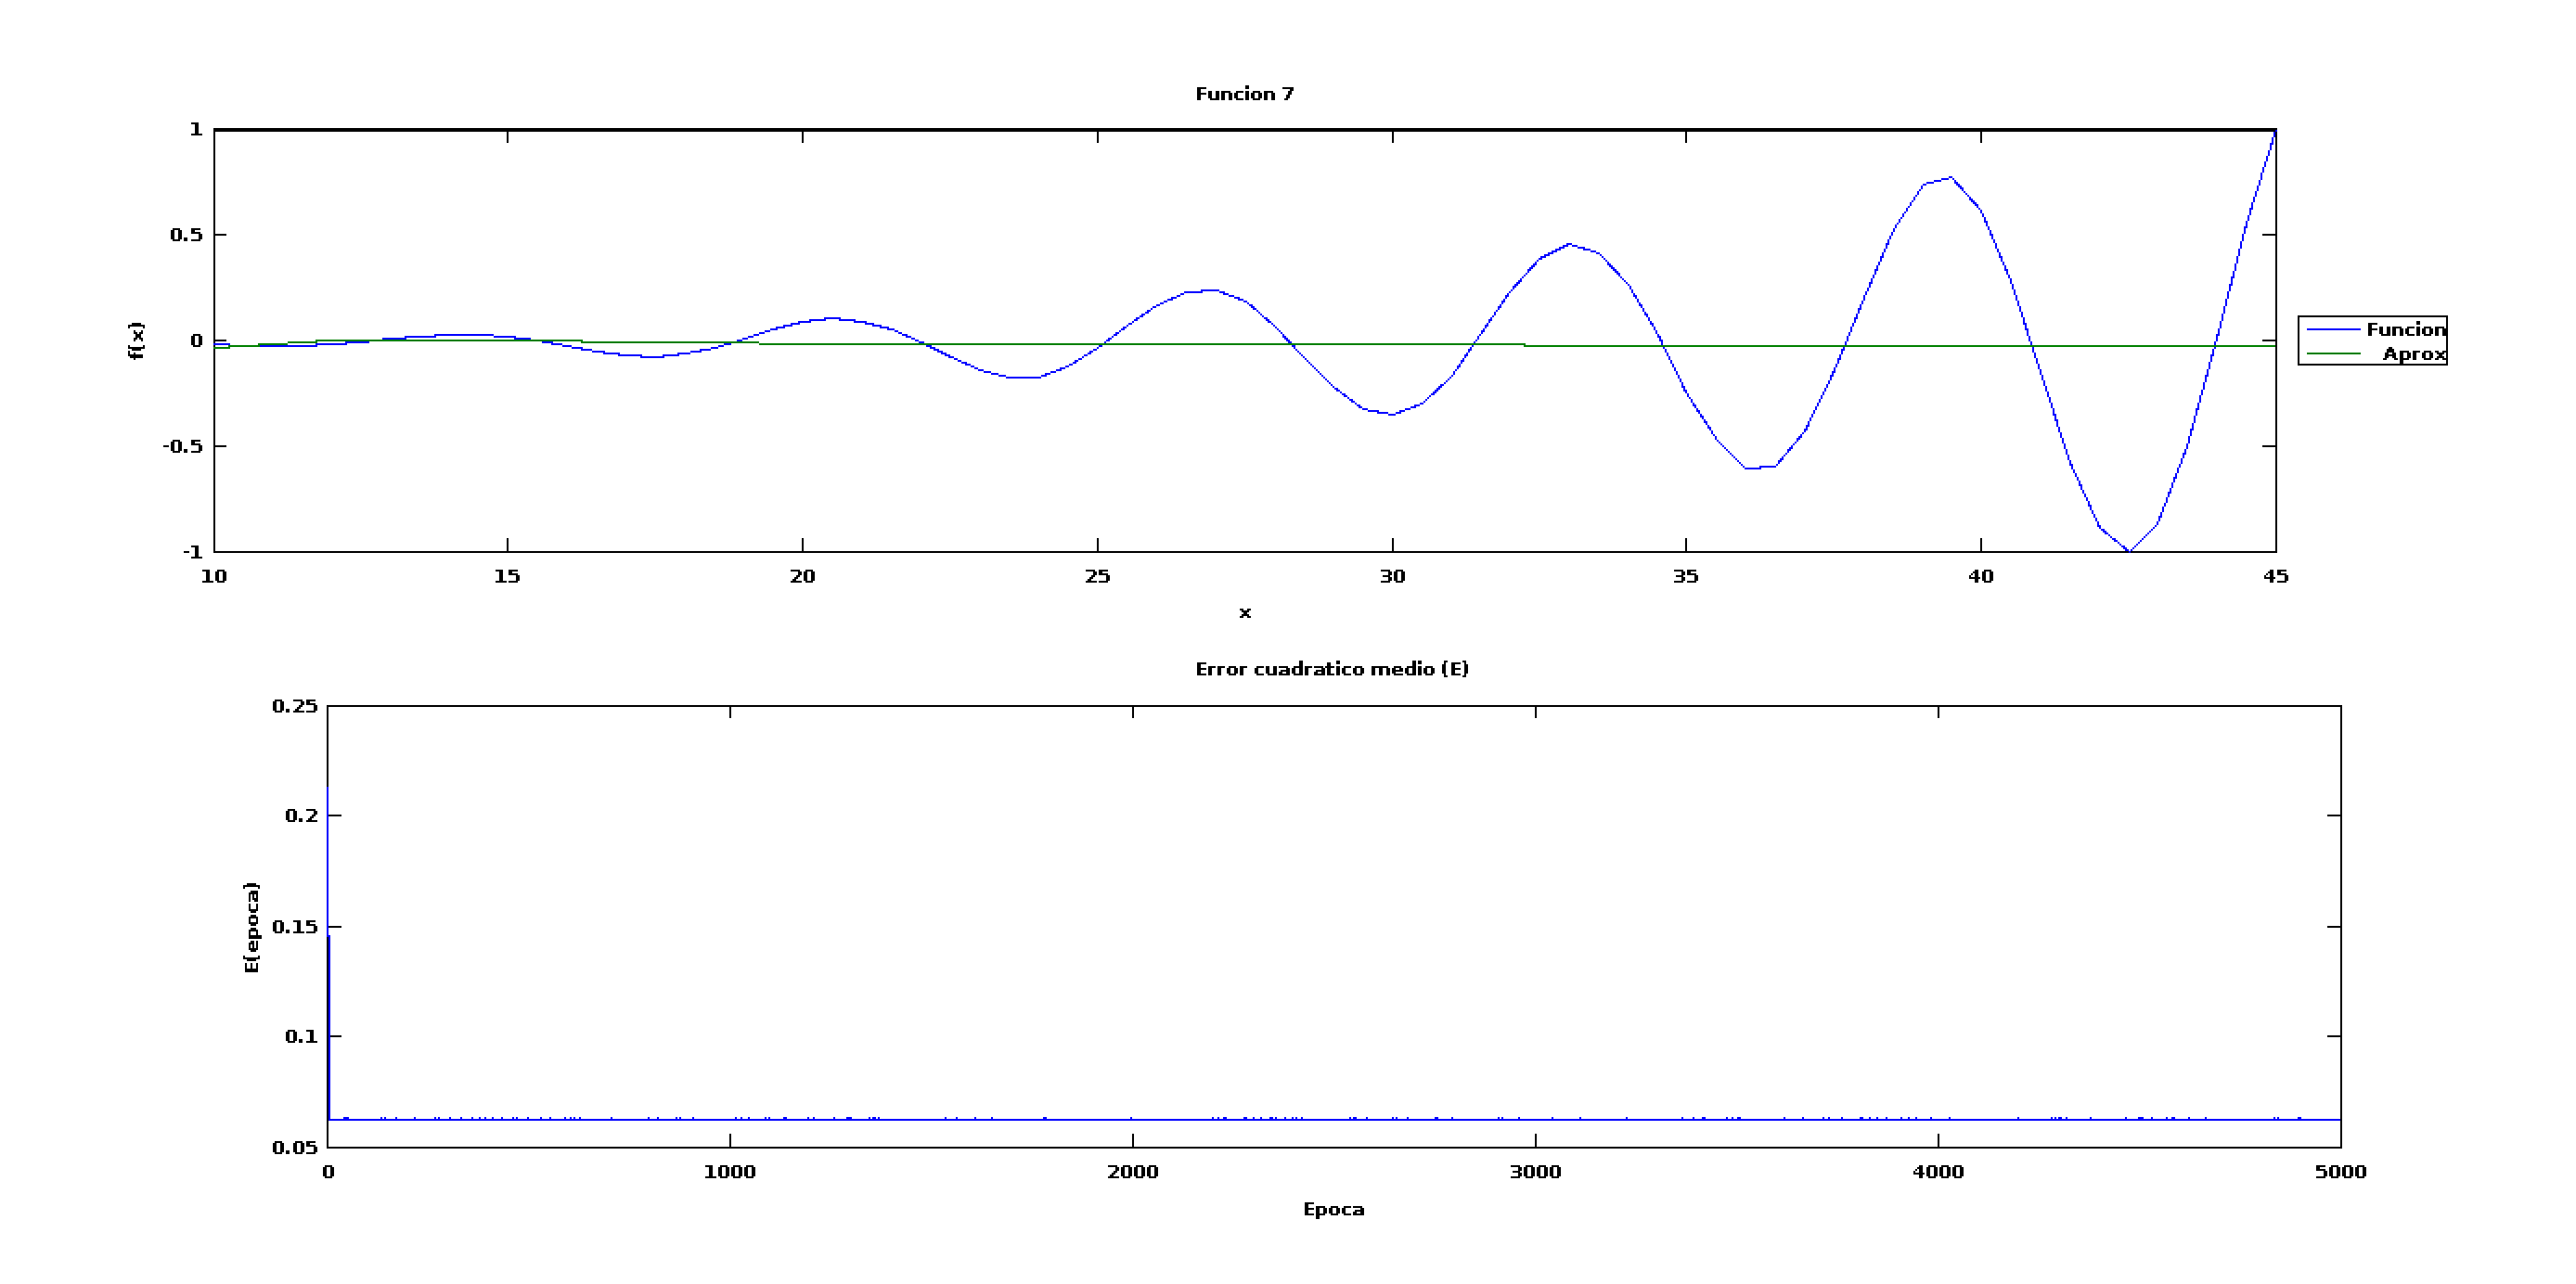
\includegraphics[width=0.85\textwidth]{img/sinNormalizar.png}
\caption{\label{fig:sinNormalizar} Prubea con la función sin normalizar \ref{table:gen}.}
\end{figure}

\begin{figure}[ht]
\centering
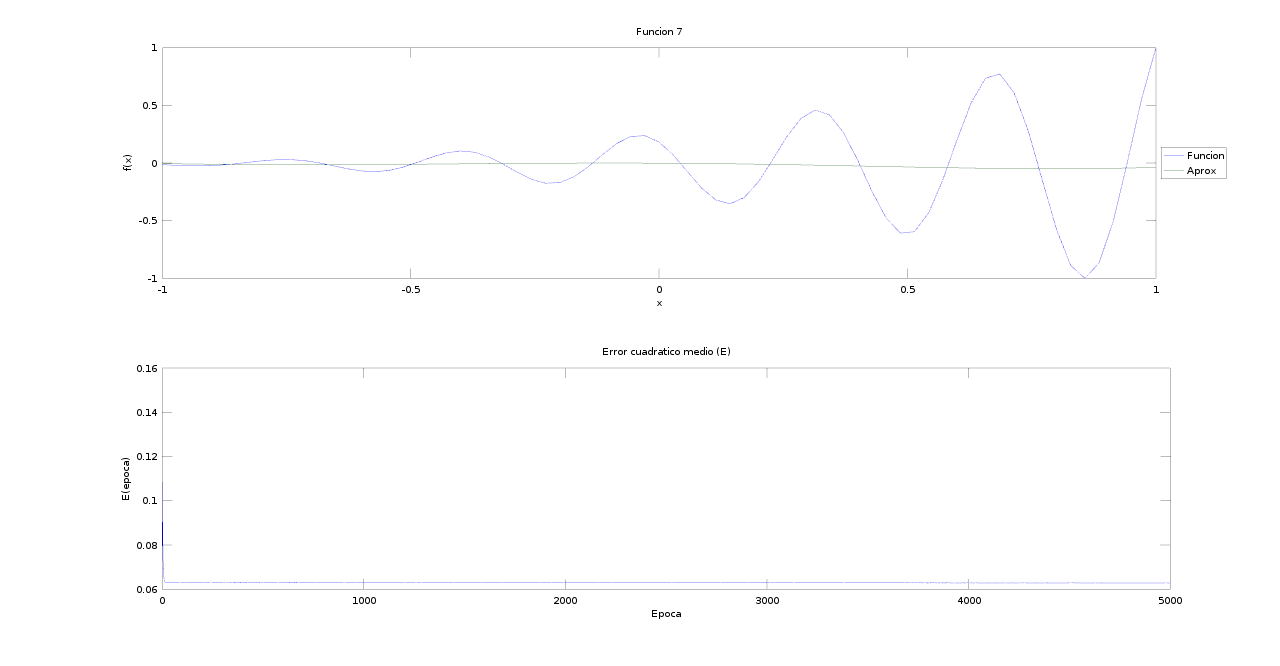
\includegraphics[width=0.85\textwidth]{img/PruebaRecu11.png}
\caption{\label{fig:PruebaRecu11} Prueba con $\beta = 1$}
\end{figure}

\begin{figure}[ht]
\centering
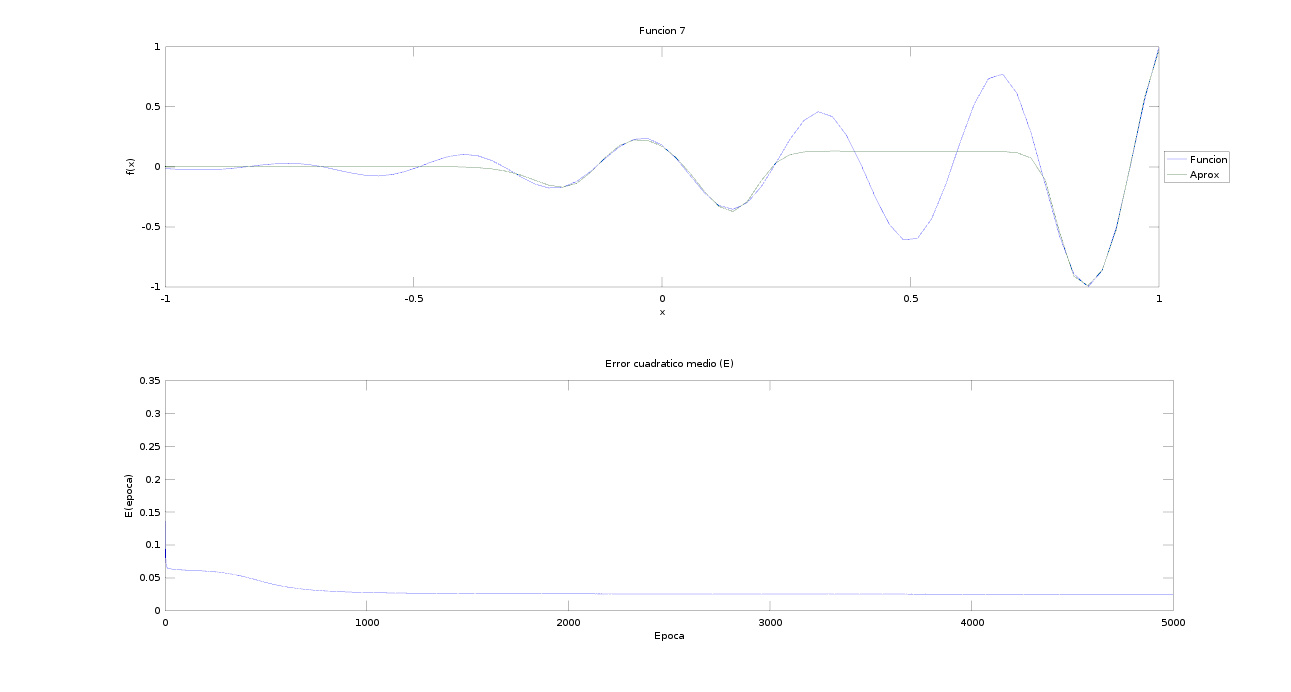
\includegraphics[width=0.85\textwidth]{img/PruebaRecu1.png}
\caption{\label{fig:pruebaRecu1} Prueba 1 de la tabla \ref{table:pruebaArqs}.}
\end{figure}

\begin{figure}[ht]
\centering
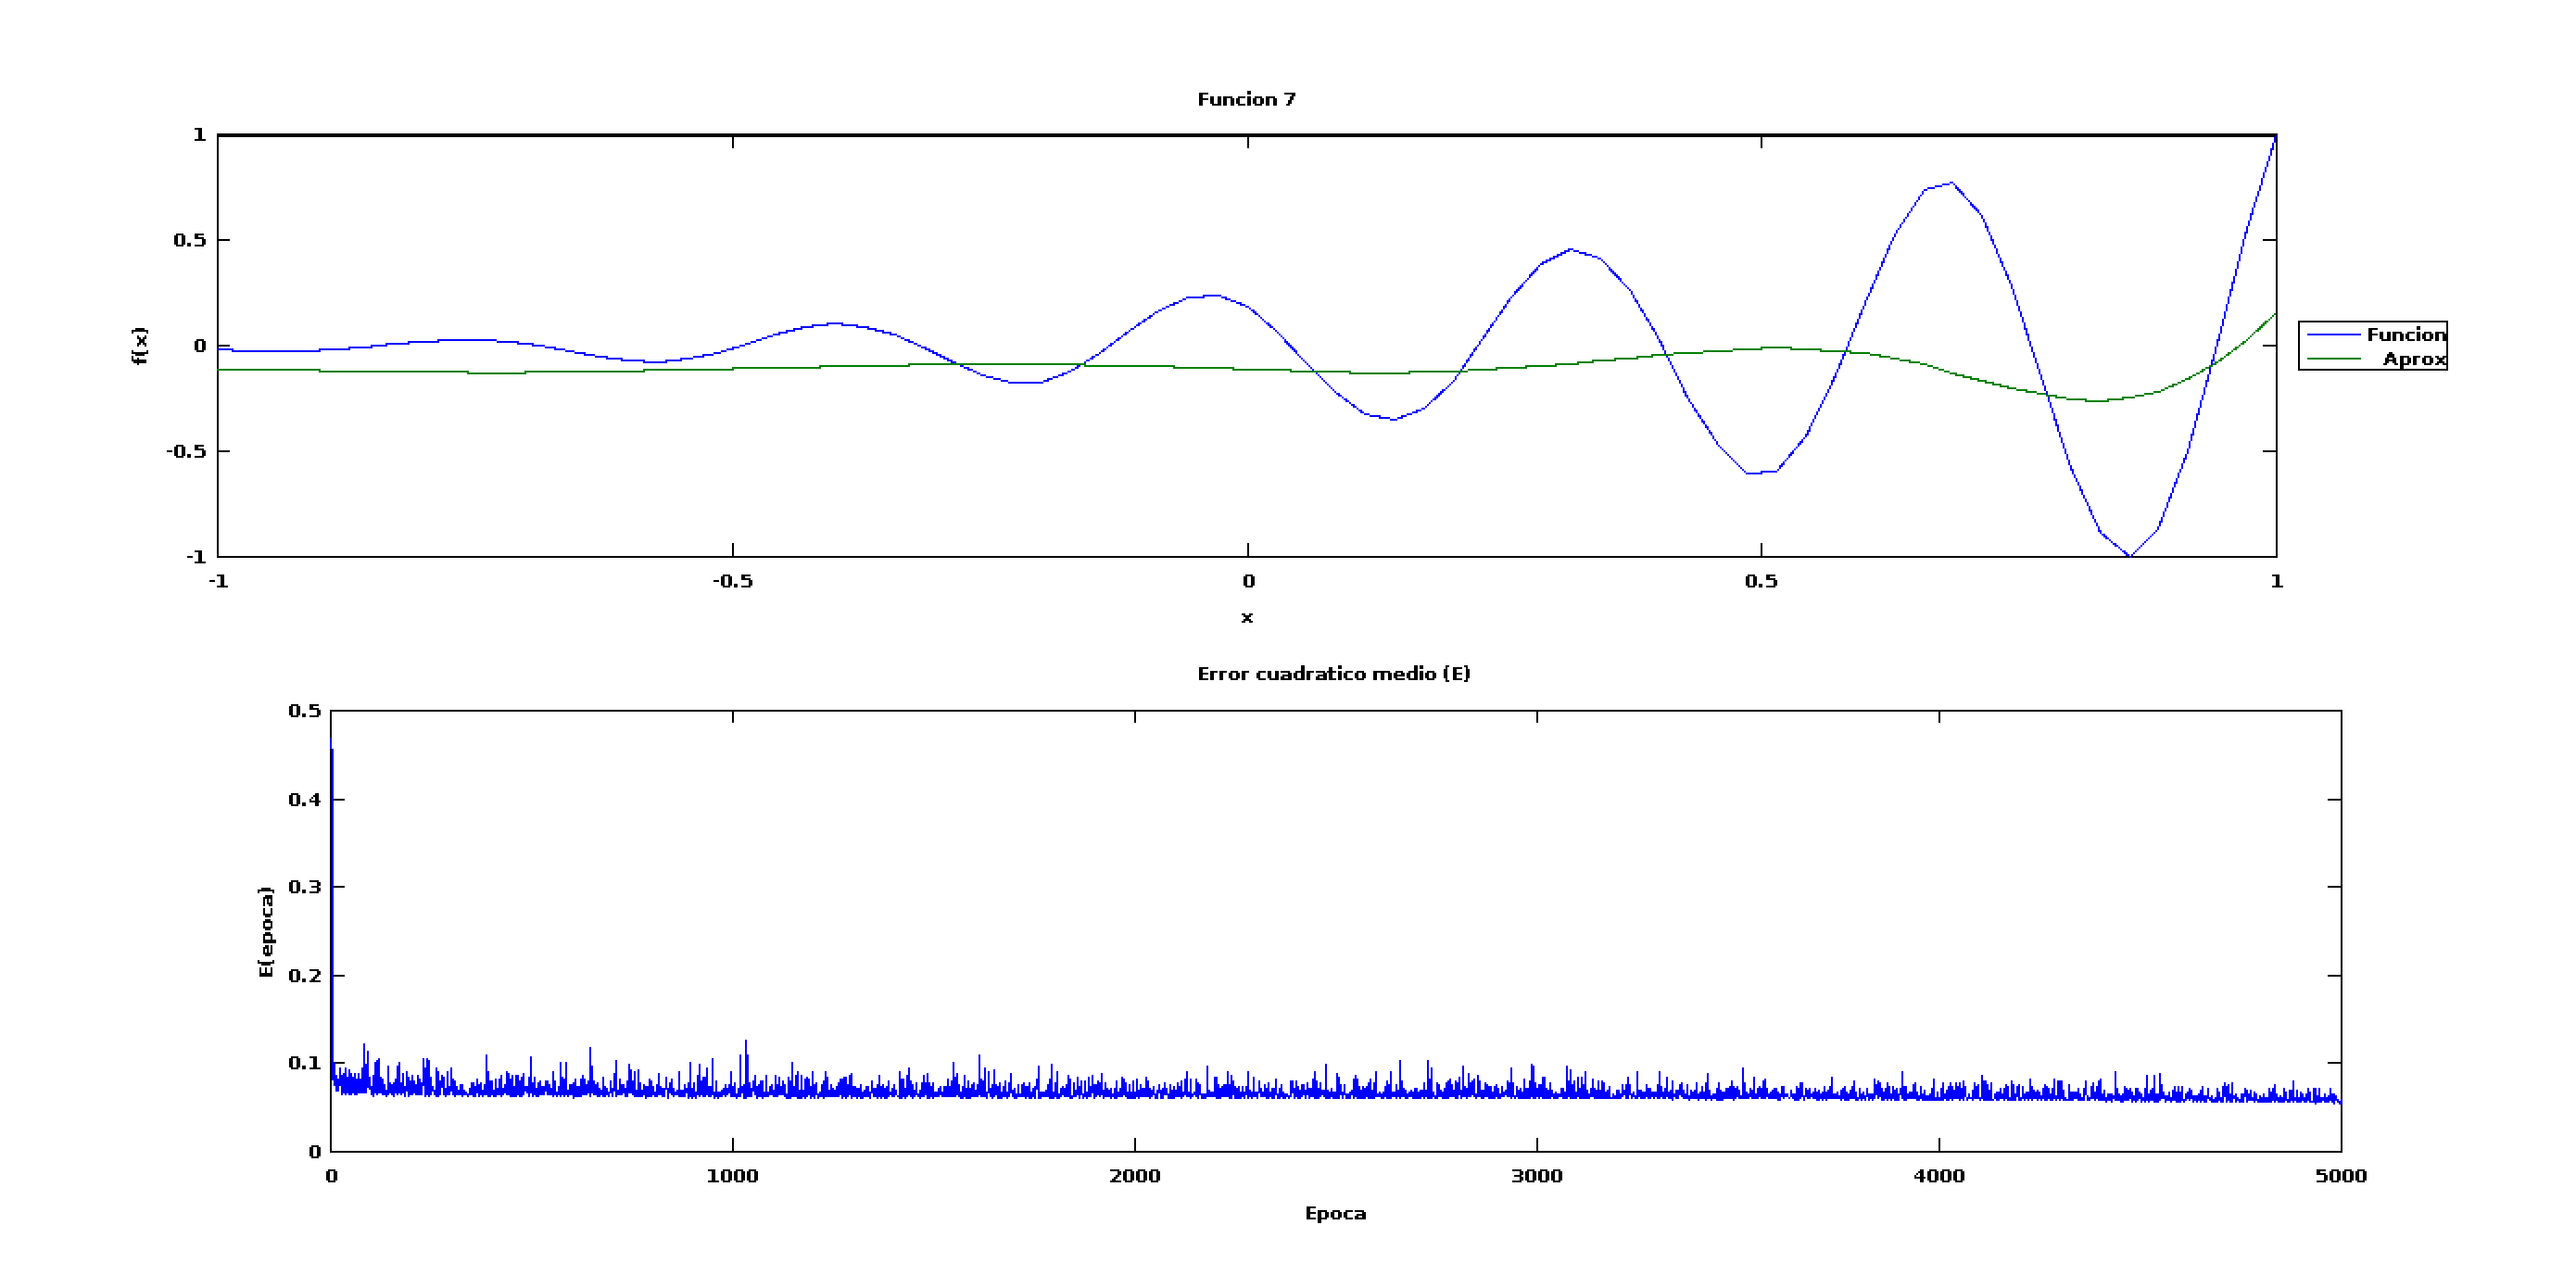
\includegraphics[width=0.85\textwidth]{img/unaCapa.png}
\caption{\label{fig:unaCapa} Prueba 13 de la tabla \ref{table:pruebaArqs}.}
\end{figure}

\begin{figure}[ht]
\centering
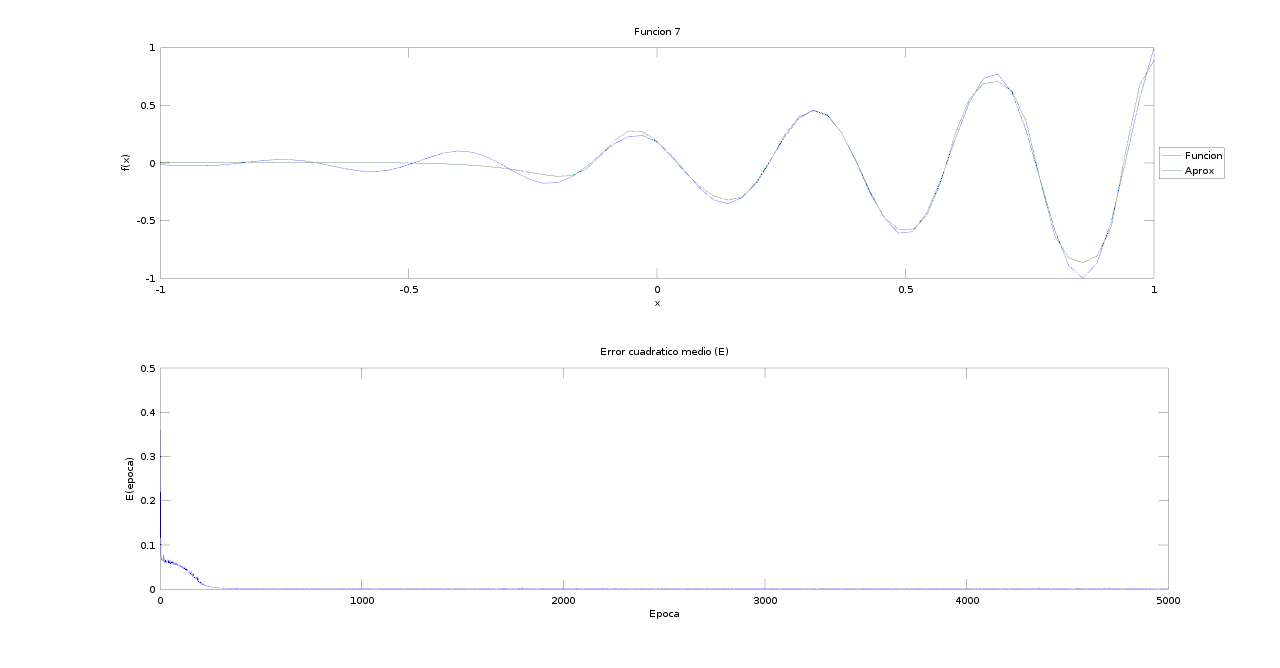
\includegraphics[width=0.85\textwidth]{img/PruebaRecu15.png}
\caption{\label{fig:pruebaRecu15} Prueba 2 de la tabla \ref{table:pruebaArqs}.}
\end{figure}

\begin{figure}[ht]
\centering
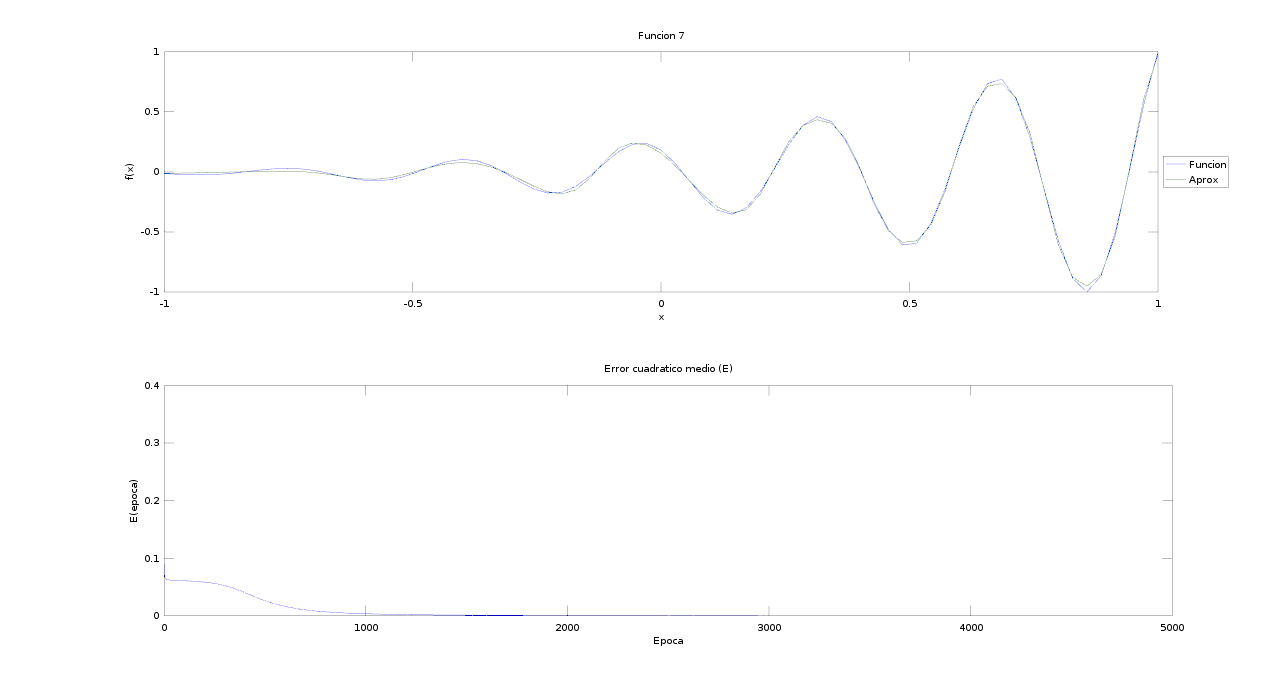
\includegraphics[width=0.85\textwidth]{img/PruebaRecu10.png}
\caption{\label{fig:pruebaRecu10} Prueba 5 de la tabla \ref{table:pruebaArqs}.}
\end{figure}

\begin{figure}[ht]
\centering
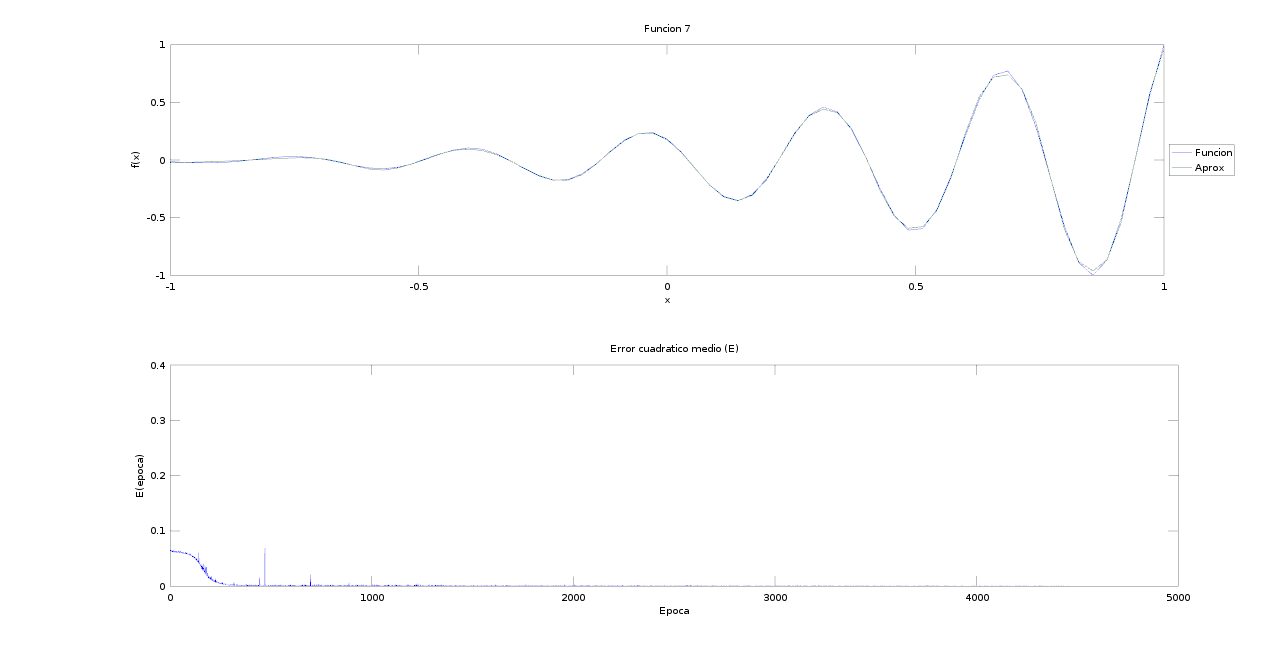
\includegraphics[width=0.85\textwidth]{img/PruebaRecu29.png}
\caption{\label{fig:pruebaRecu29} Prueba 1 de la tabla \ref{table:pruebaEta}.}
\end{figure}

\begin{figure}[ht]
\centering
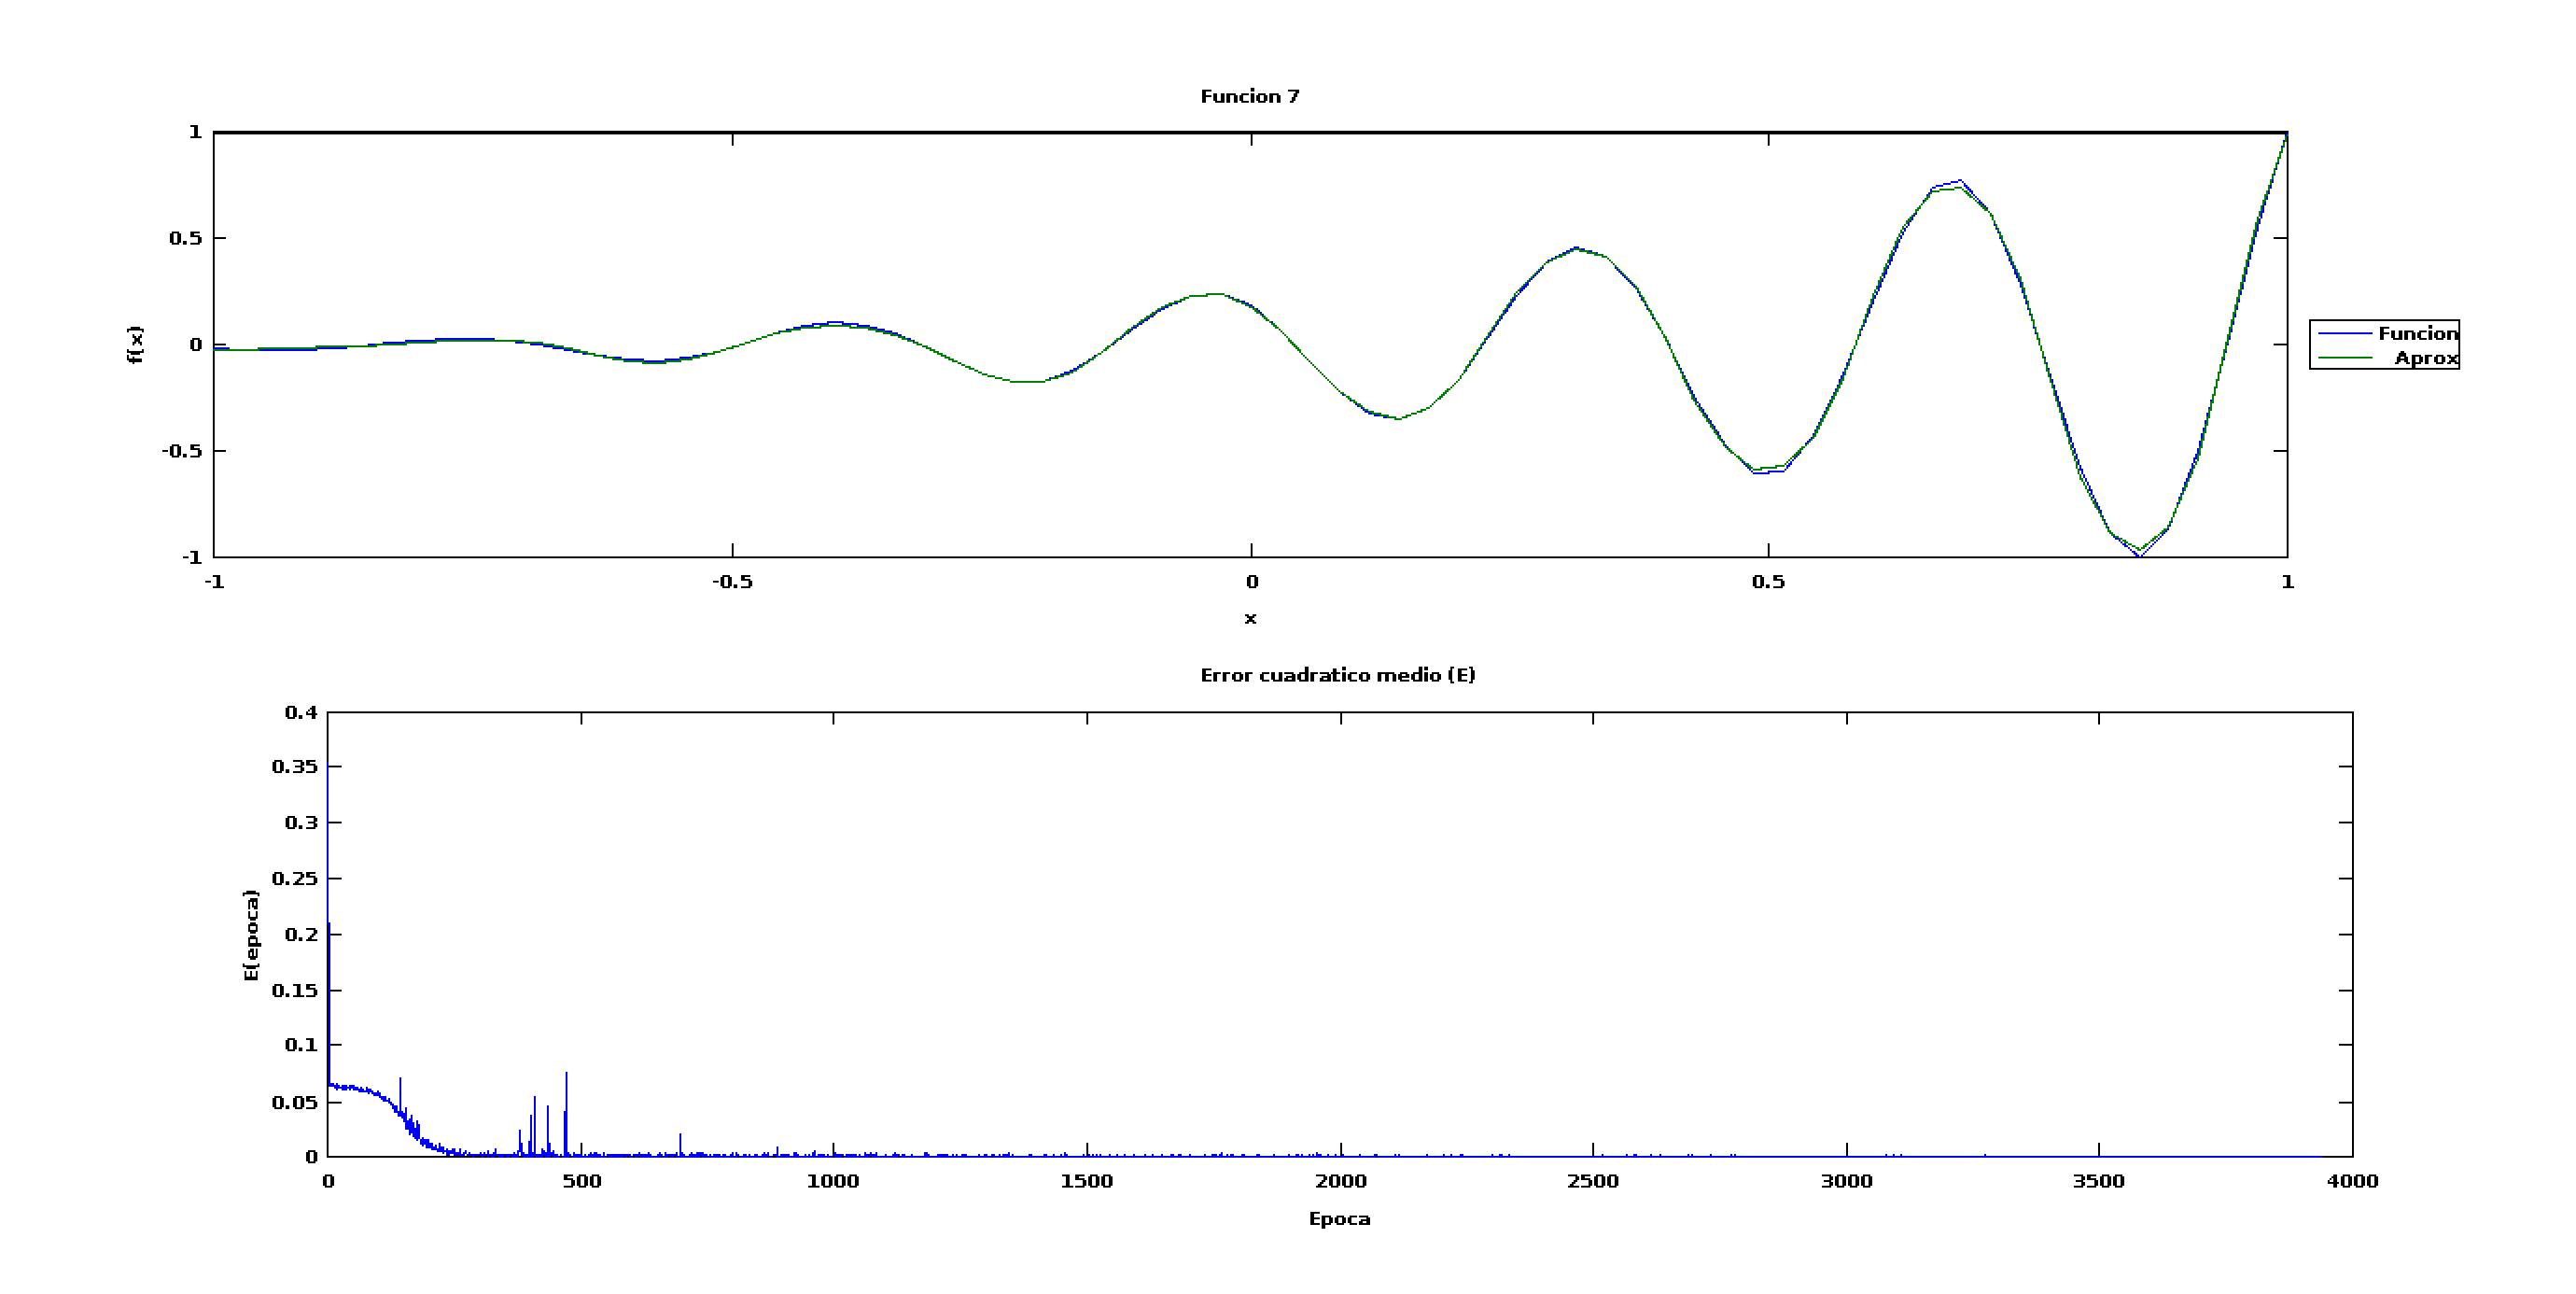
\includegraphics[width=0.85\textwidth]{img/PruebaRecu40.png}
\caption{\label{fig:pruebaRecu40} Prueba 1 de la tabla \ref{table:pruebaMomentum}.}
\end{figure}

\begin{figure}[ht]
\centering
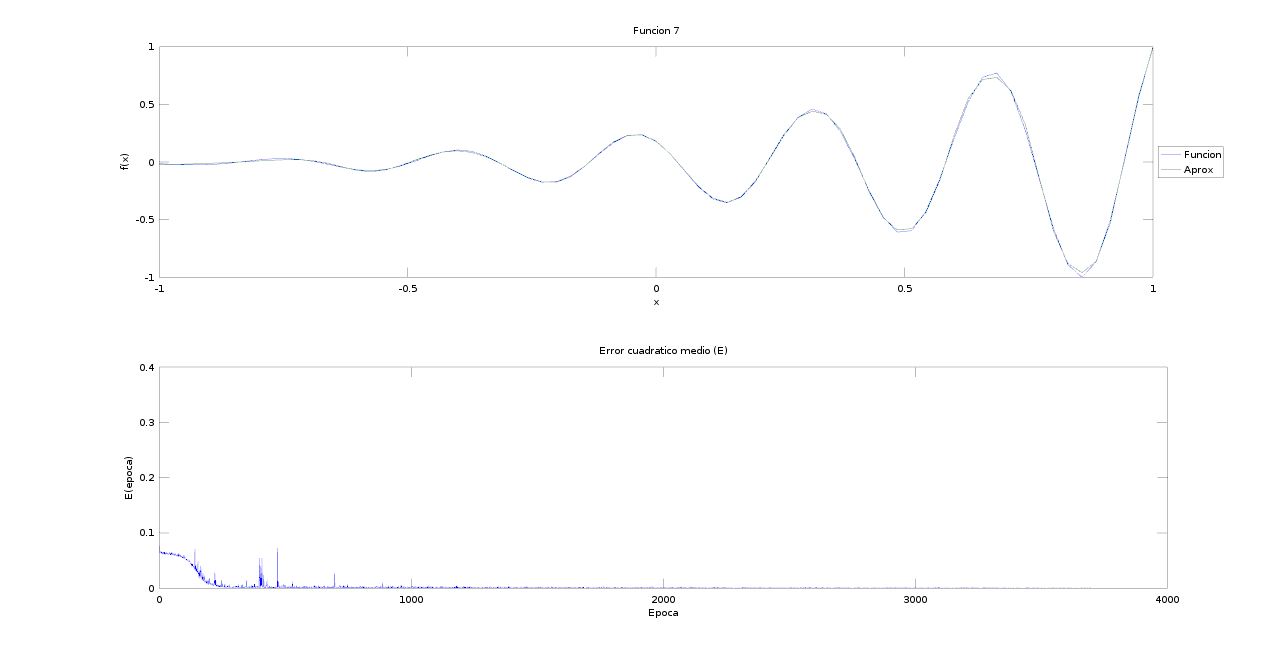
\includegraphics[width=0.85\textwidth]{img/PruebaRecu25.png}
\caption{\label{fig:pruebaRecu25} Prueba 2 de la tabla \ref{table:pruebaMomentum}.}
\end{figure}

\begin{figure}[ht]
\centering
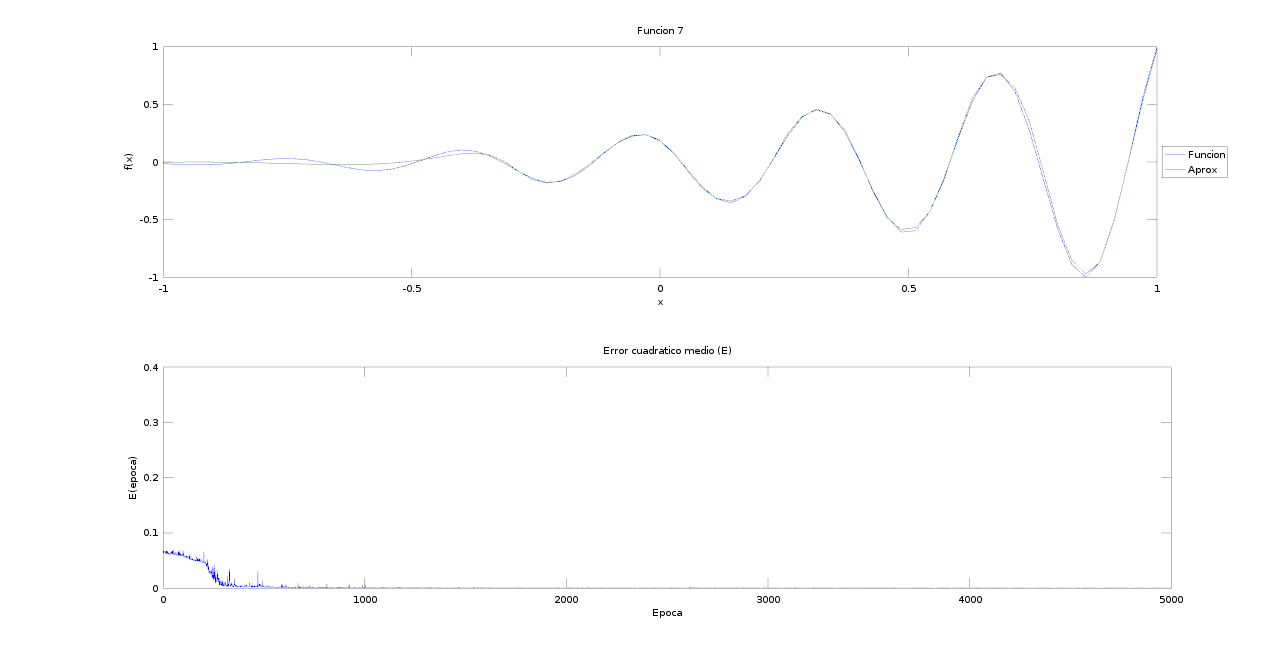
\includegraphics[width=0.85\textwidth]{img/PruebaRecu26.png}
\caption{\label{fig:pruebaRecu26} Prueba 3 de la tabla \ref{table:pruebaMomentum}.}
\end{figure}

\clearpage


\begin{figure}[ht]
\centering
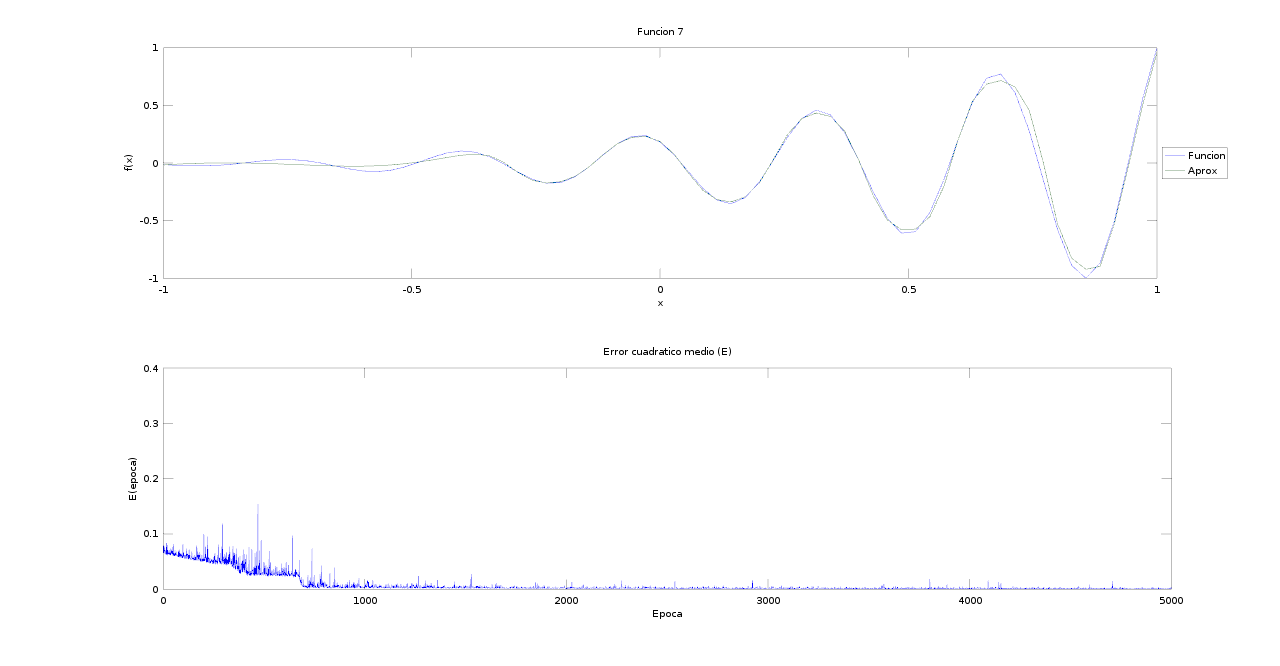
\includegraphics[width=0.85\textwidth]{img/PruebaRecu27.png}
\caption{\label{fig:pruebaRecu27} Prueba 4 de la tabla \ref{table:pruebaMomentum}.}
\end{figure}


\begin{figure}[ht]
\centering
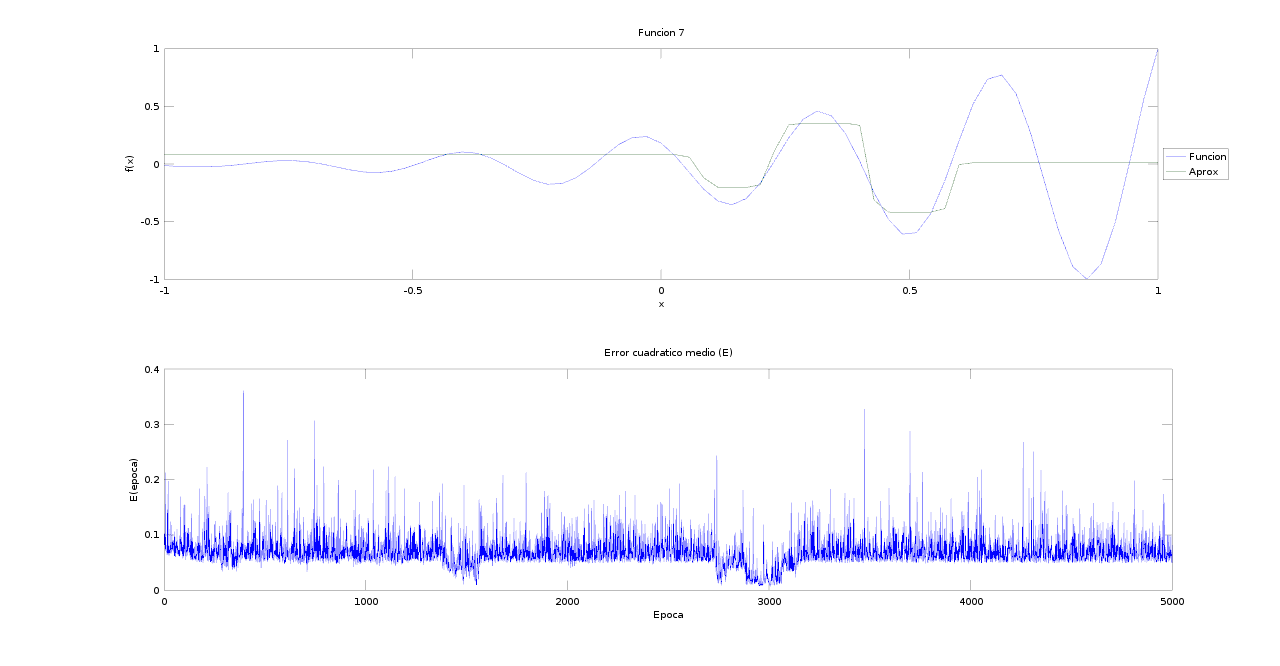
\includegraphics[width=0.85\textwidth]{img/PruebaRecu28.png}
\caption{\label{fig:pruebaRecu28} Prueba 5 de la tabla \ref{table:pruebaMomentum}.}
\end{figure}

\begin{figure}[ht]
\centering
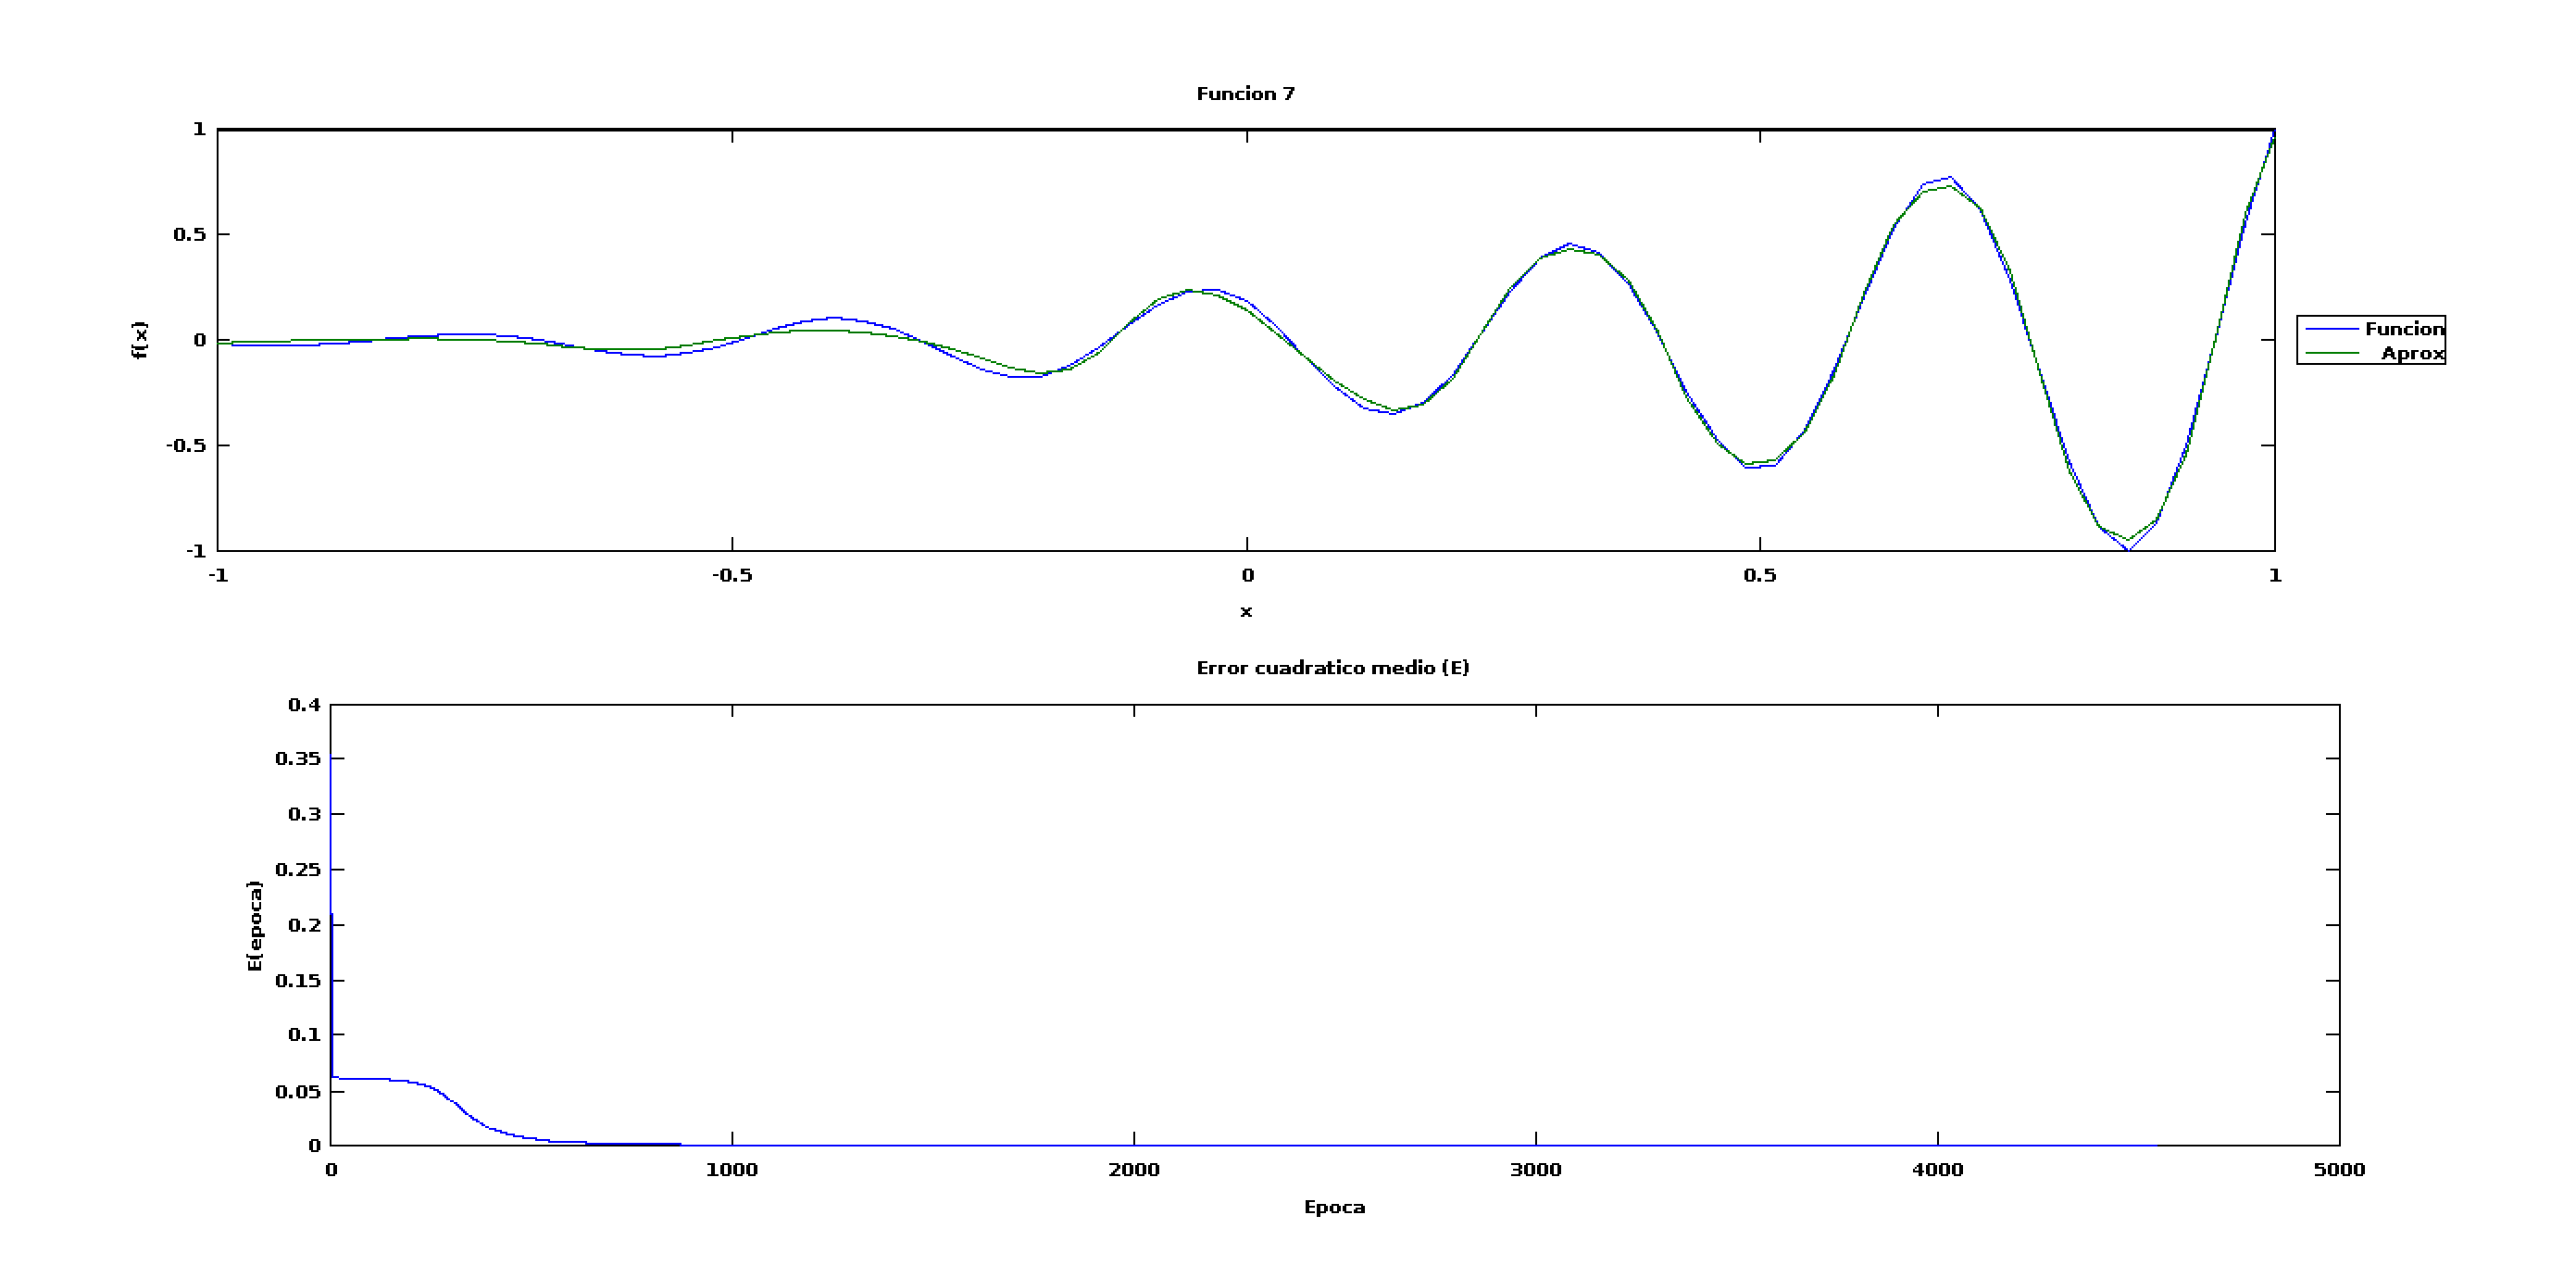
\includegraphics[width=0.85\textwidth]{img/PruebaRecu39.png}
\caption{\label{fig:pruebaRecu39} Prueba 4 de la tabla \ref{table:pruebaEtaAdapt}.}
\end{figure}


\begin{figure}[ht]
\centering
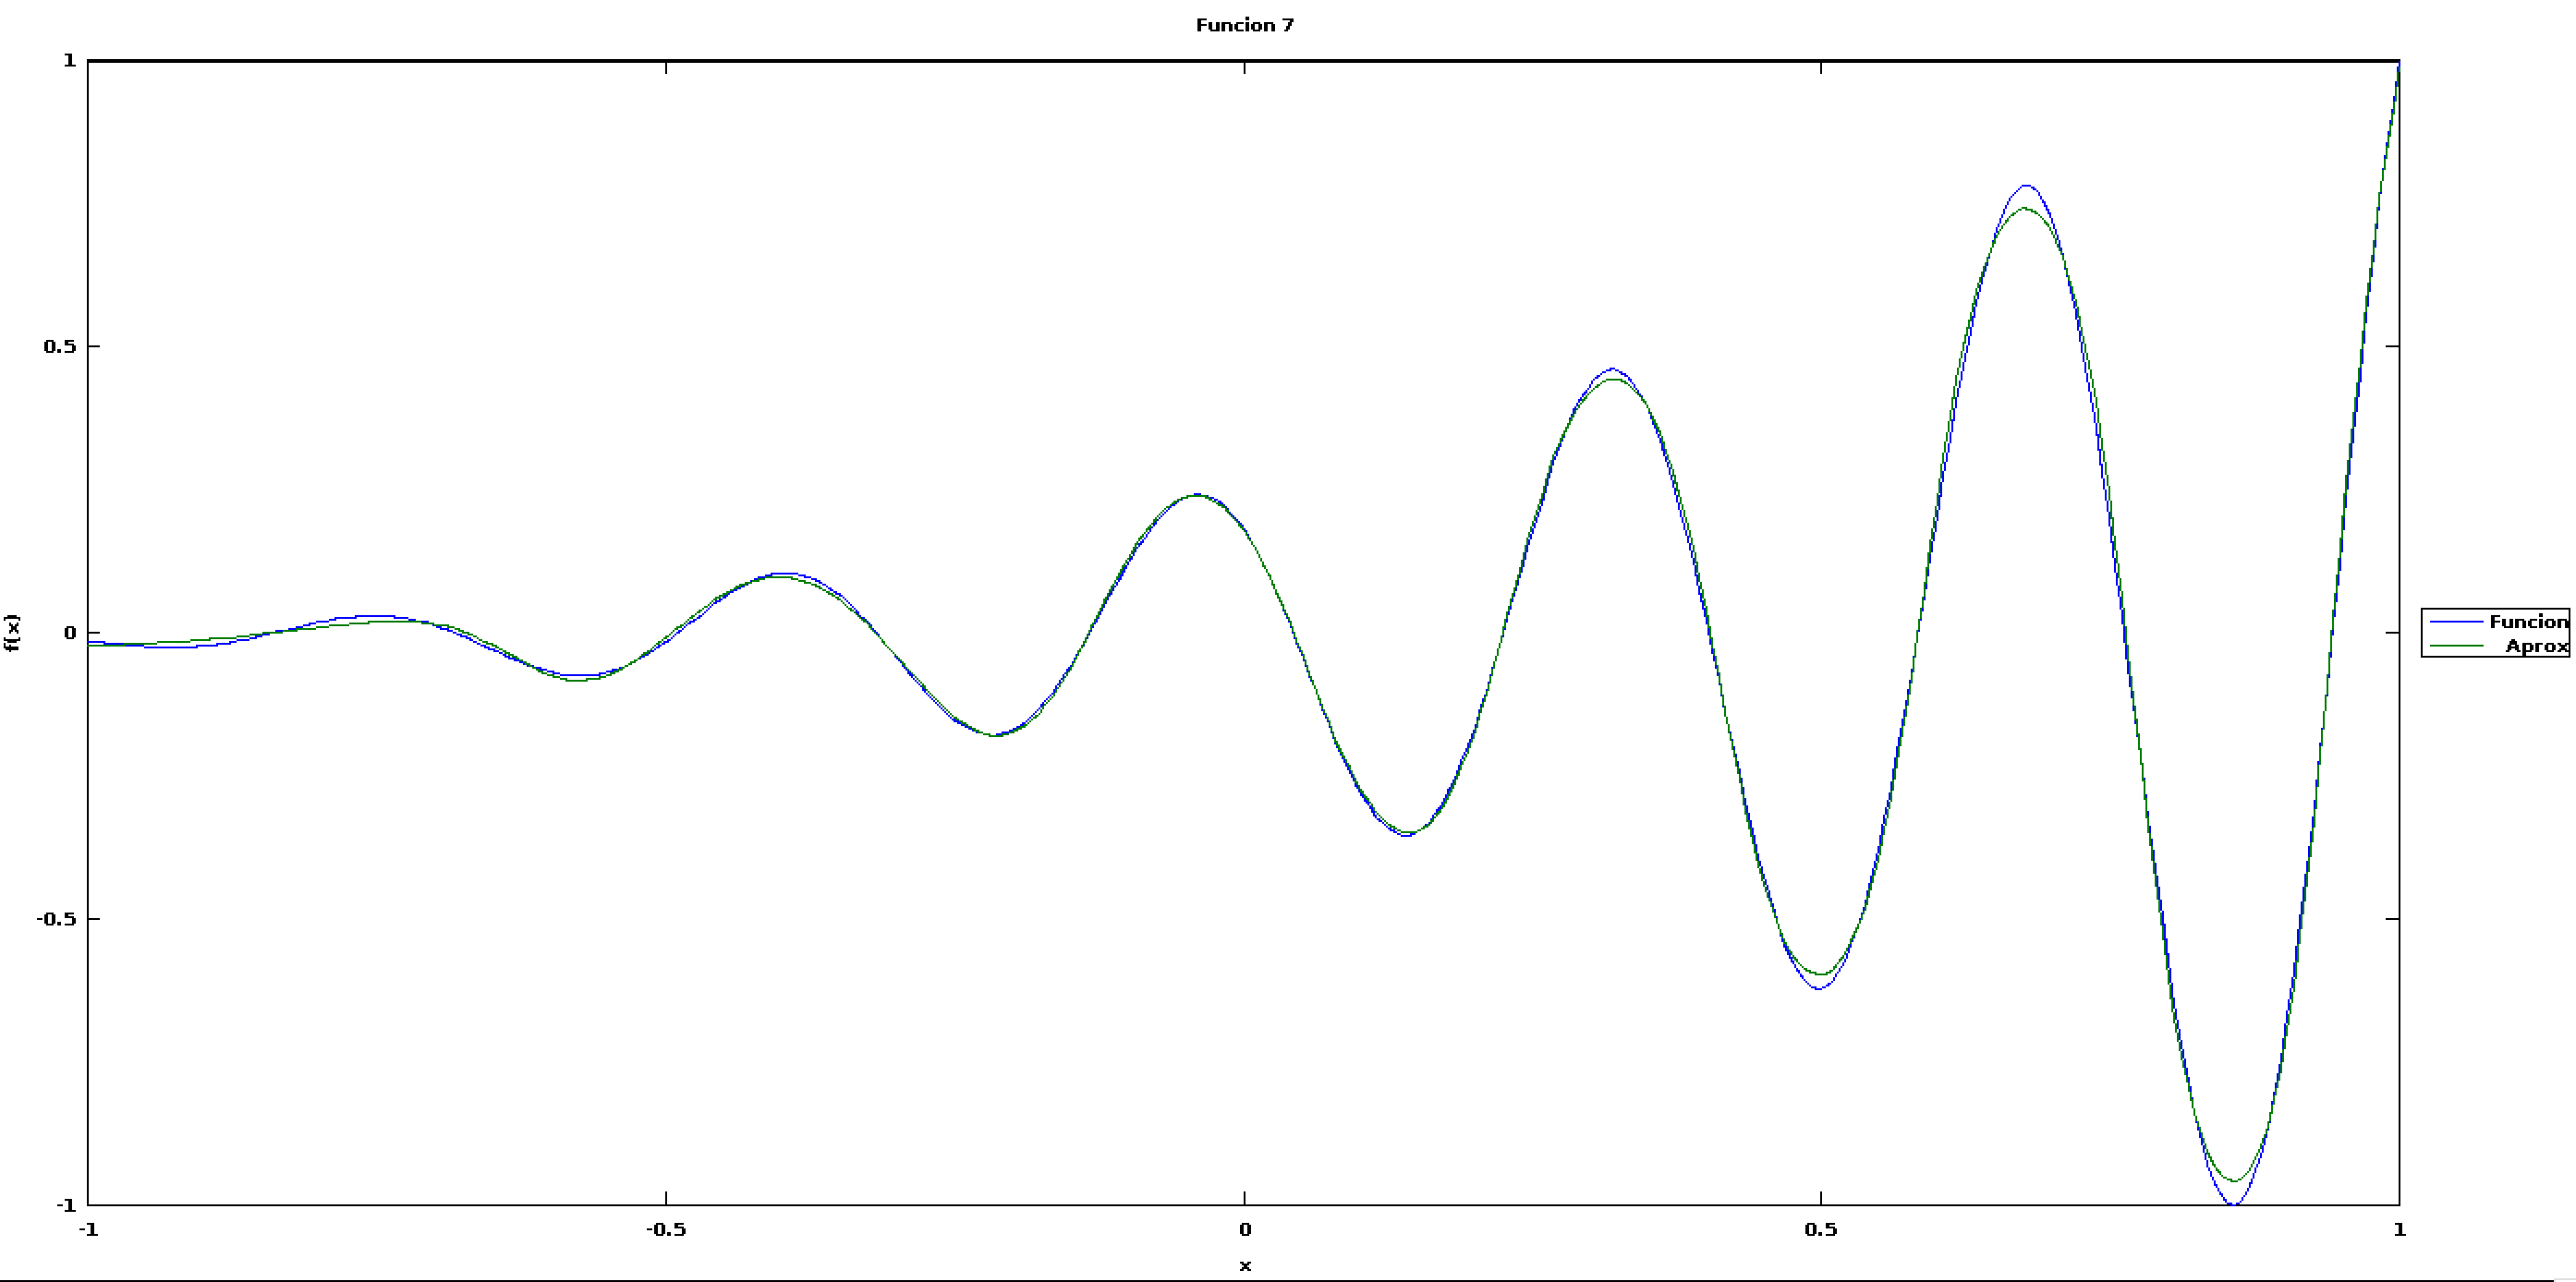
\includegraphics[width=0.85\textwidth]{img/gen1.png}
\caption{\label{fig:gen1} Generalización 1 de la tabla \ref{table:gen}. Incremento $= 0.1$}
\end{figure}

\begin{figure}[ht]
\centering
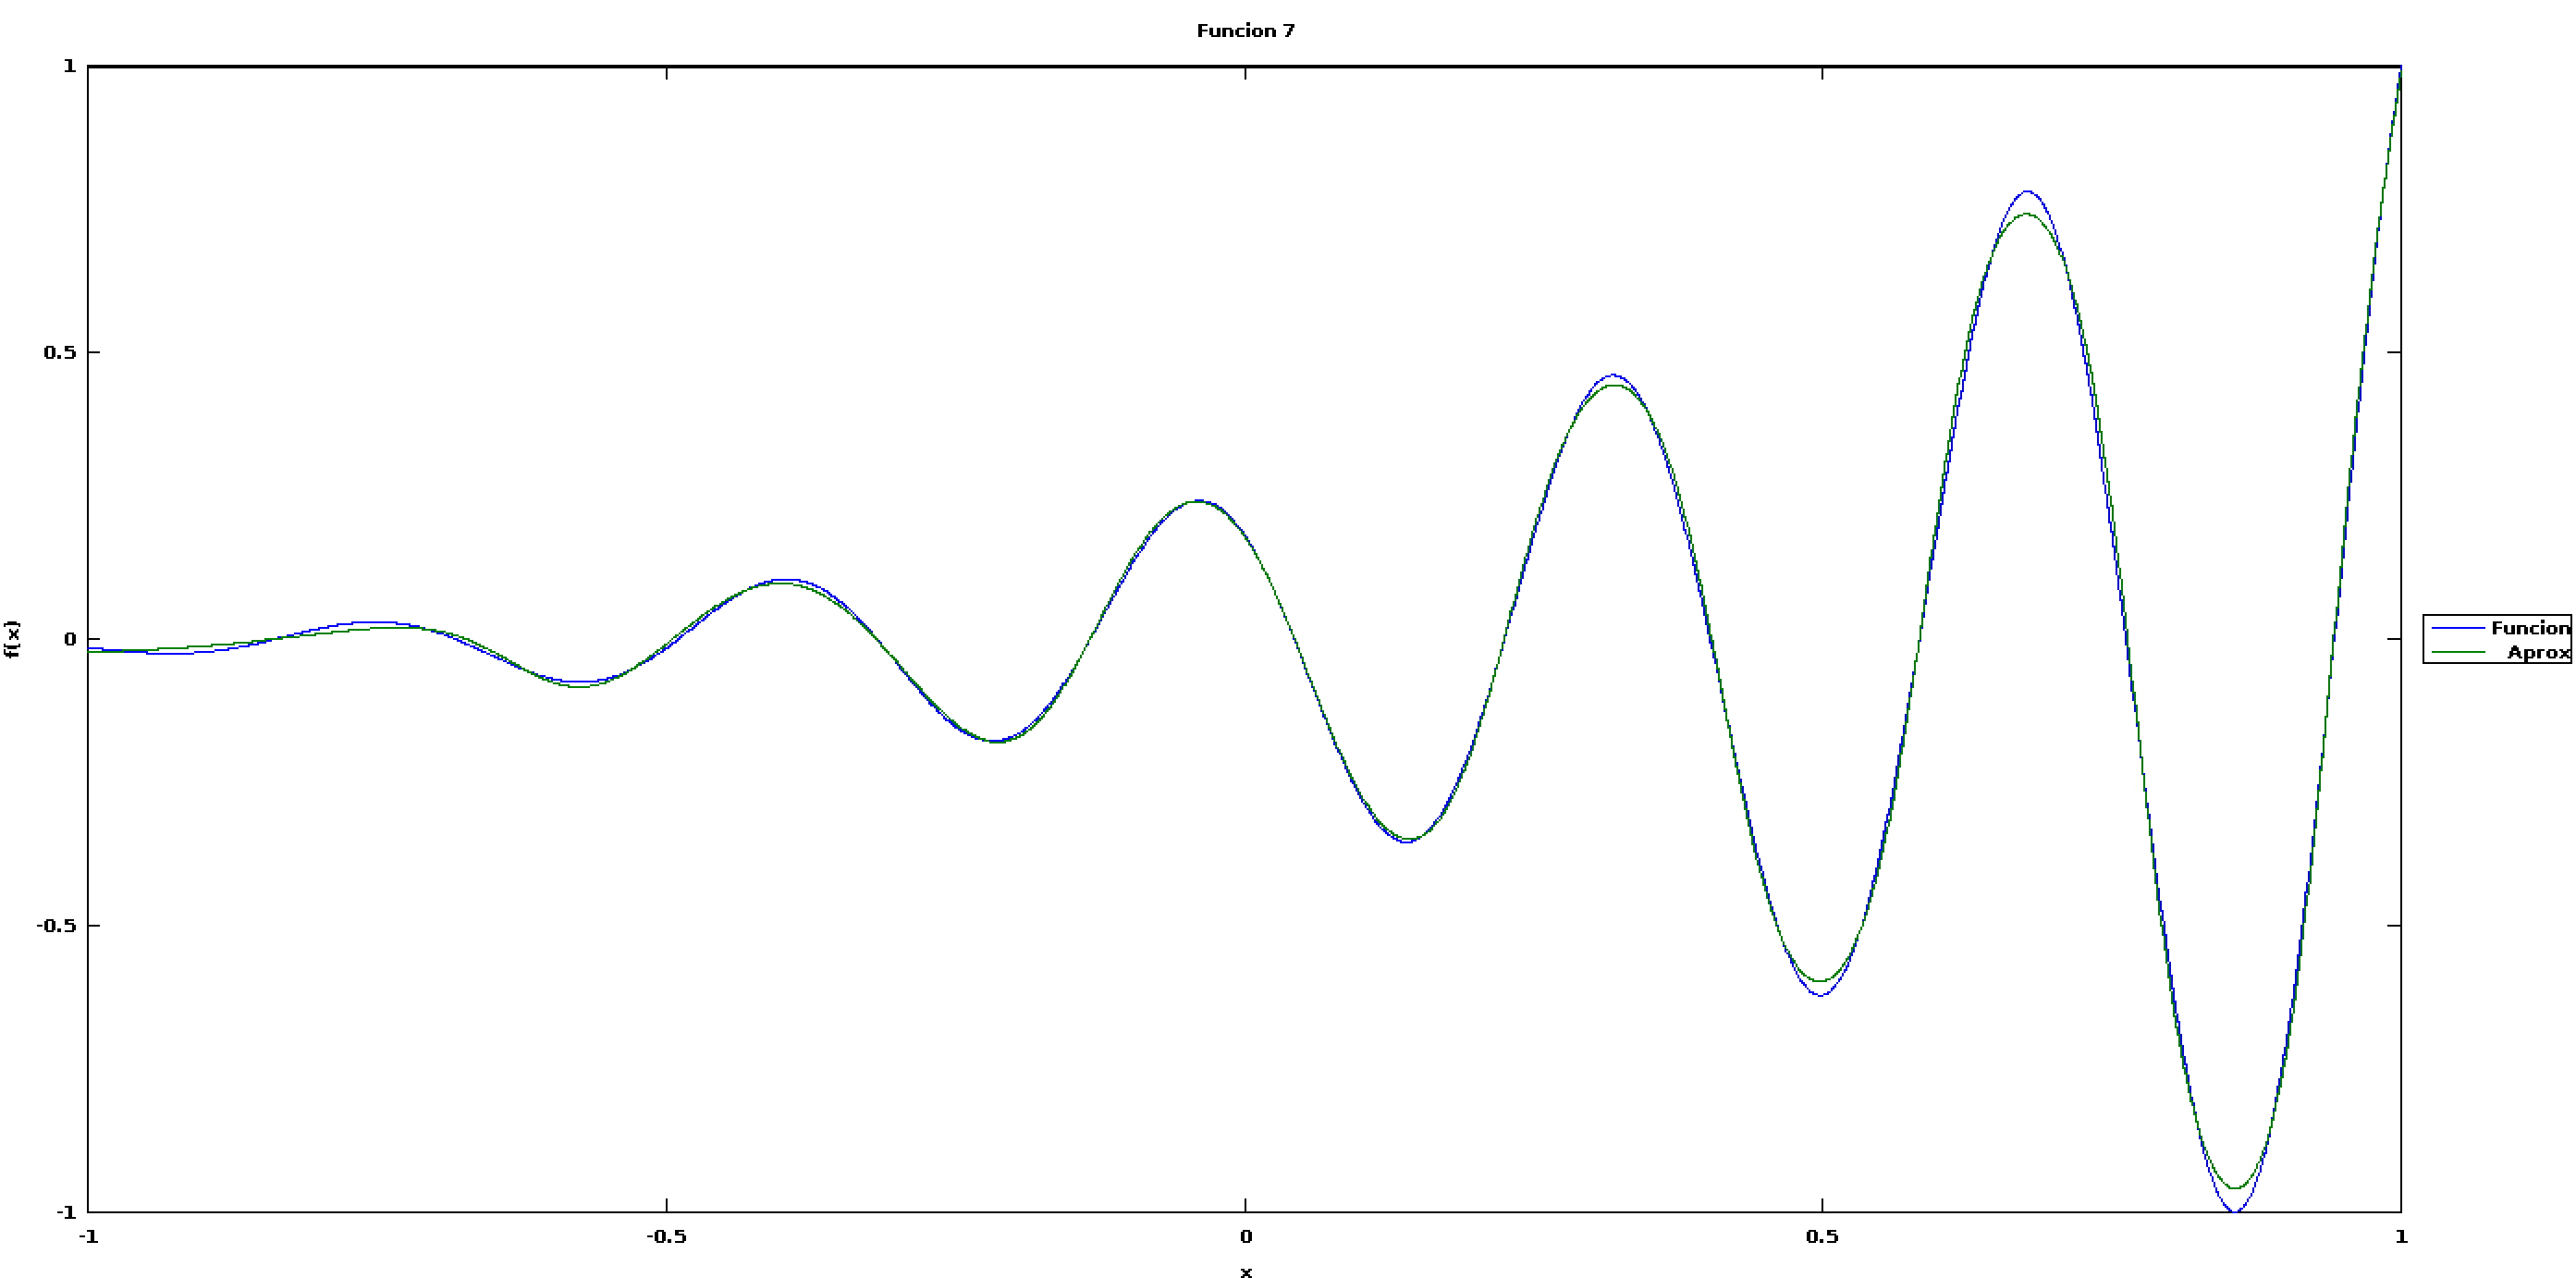
\includegraphics[width=0.85\textwidth]{img/gen2.png}
\caption{\label{fig:gen2} Generalización 2 de la tabla \ref{table:gen}. Incremento $= 0.01$}
\end{figure}

\begin{figure}[ht]
\centering
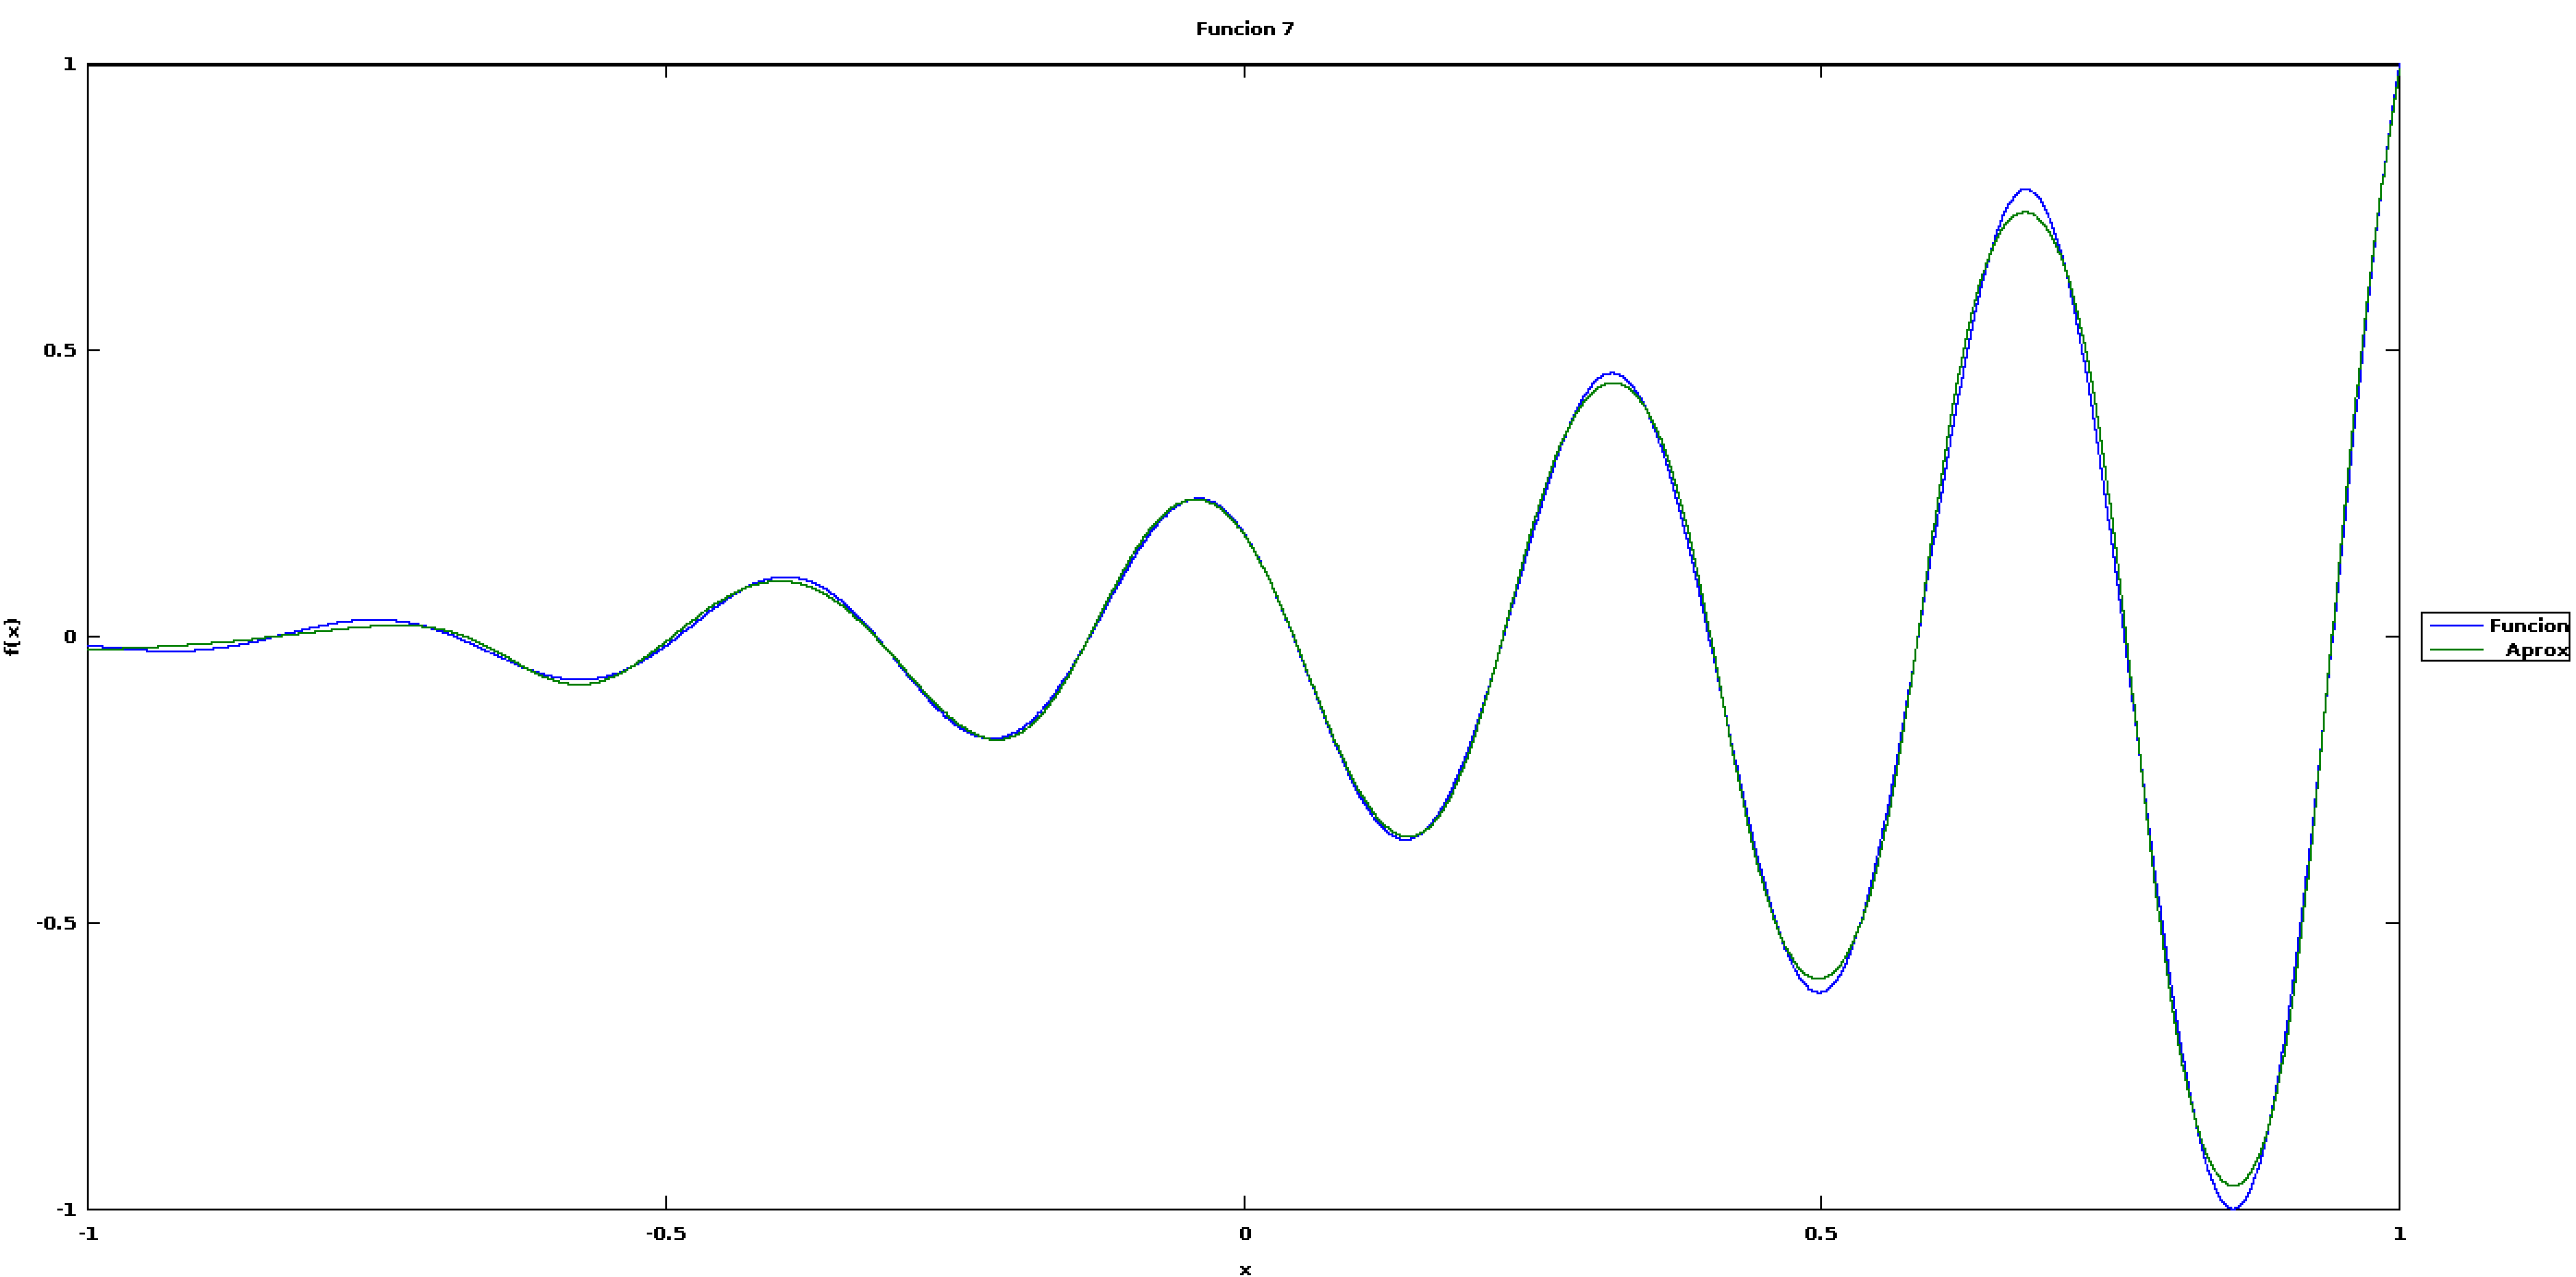
\includegraphics[width=0.85\textwidth]{img/gen3.png}
\caption{\label{fig:gen3} Generalización 3 de la tabla \ref{table:gen}. Incremento $= 0.001$}
\end{figure}

\end{document}